\documentclass[11pt,fleqn]{book} % Default font size and left-justified equations

%----------------------------------------------------------------------------------------

\usepackage{longtable}
\usepackage{array}
%%%%%%%%%%%%%%%%%%%%%%%%%%%%%%%%%%%%%%%%%
% The Legrand Orange Book
% Structural Definitions File
% Version 2.0 (9/2/15)
%
% Original author:
% Mathias Legrand (legrand.mathias@gmail.com) with modifications by:
% Vel (vel@latextemplates.com)
% 
% This file has been downloaded from:	
% http://www.LaTeXTemplates.com
%
% License:
% CC BY-NC-SA 3.0 (http://creativecommons.org/licenses/by-nc-sa/3.0/)
%
%%%%%%%%%%%%%%%%%%%%%%%%%%%%%%%%%%%%%%%%%

%----------------------------------------------------------------------------------------
%	VARIOUS REQUIRED PACKAGES AND CONFIGURATIONS
%----------------------------------------------------------------------------------------

\usepackage[top=3cm,bottom=3cm,left=3cm,right=3cm,headsep=10pt,a4paper]{geometry} % Page margins

\usepackage{graphicx} % Required for including pictures
\graphicspath{{Pictures/}} % Specifies the directory where pictures are stored

\usepackage{lipsum} % Inserts dummy text

\usepackage{tikz} % Required for drawing custom shapes

\usepackage[spanish]{babel} % English language/hyphenation

\usepackage{enumitem} % Customize lists
\setlist{nolistsep} % Reduce spacing between bullet points and numbered lists

\usepackage{booktabs} % Required for nicer horizontal rules in tables

\usepackage{xcolor} % Required for specifying colors by name
%\definecolor{ocre}{RGB}{243,102,25} % Define the orange color used for highlighting throughout the book
\definecolor{ocre}{RGB}{89,65,203} % Define the orange color used for 
%----------------------------------------------------------------------------------------
%	FONTS
%----------------------------------------------------------------------------------------

\usepackage{avant} % Use the Avantgarde font for headings
%\usepackage{times} % Use the Times font for headings
\usepackage{mathptmx} % Use the Adobe Times Roman as the default text font together with math symbols from the Sym­bol, Chancery and Com­puter Modern fonts

\usepackage{microtype} % Slightly tweak font spacing for aesthetics
\usepackage[utf8]{inputenc} % Required for including letters with accents
\usepackage[T1]{fontenc} % Use 8-bit encoding that has 256 glyphs

%----------------------------------------------------------------------------------------
%	BIBLIOGRAPHY AND INDEX
%----------------------------------------------------------------------------------------
%\usepackage[style=alphabetic,citestyle=numeric,sorting=nyt,sortcites=true,autopunct=true,babel=hyphen,hyperref=true,abbreviate=false,backref=true,backend=biber]{biblatex}
%\addbibresource{bibliography.bib} % BibTeX bibliography file
%\defbibheading{bibempty}{}

\usepackage{calc} % For simpler calculation - used for spacing the index letter headings correctly
\usepackage{makeidx} % Required to make an index
\makeindex % Tells LaTeX to create the files required for indexing

%----------------------------------------------------------------------------------------
%	MAIN TABLE OF CONTENTS
%----------------------------------------------------------------------------------------

\usepackage{titletoc} % Required for manipulating the table of contents

\contentsmargin{0cm} % Removes the default margin

% Part text styling
\titlecontents{part}[0cm]
{\addvspace{20pt}\centering\large\bfseries}
{}
{}
{}

% Chapter text styling
\titlecontents{chapter}[1.25cm] % Indentation
{\addvspace{12pt}\large\sffamily\bfseries} % Spacing and font options for chapters
{\color{ocre!60}\contentslabel[\Large\thecontentslabel]{1.25cm}\color{ocre}} % Chapter number
{\color{ocre}}  
{\color{ocre!60}\normalsize\;\titlerule*[.5pc]{.}\;\thecontentspage} % Page number

% Section text styling
\titlecontents{section}[1.25cm] % Indentation
{\addvspace{3pt}\sffamily\bfseries} % Spacing and font options for sections
{\contentslabel[\thecontentslabel]{1.25cm}} % Section number
{}
{\hfill\color{black}\thecontentspage} % Page number
[]

% Subsection text styling
\titlecontents{subsection}[1.25cm] % Indentation
{\addvspace{1pt}\sffamily\small} % Spacing and font options for subsections
{\contentslabel[\thecontentslabel]{1.25cm}} % Subsection number
{}
{\ \titlerule*[.5pc]{.}\;\thecontentspage} % Page number
[]

% List of figures
\titlecontents{figure}[0em]
{\addvspace{-5pt}\sffamily}
{\thecontentslabel\hspace*{1em}}
{}
{\ \titlerule*[.5pc]{.}\;\thecontentspage}
[]

% List of tables
\titlecontents{table}[0em]
{\addvspace{-5pt}\sffamily}
{\thecontentslabel\hspace*{1em}}
{}
{\ \titlerule*[.5pc]{.}\;\thecontentspage}
[]

%----------------------------------------------------------------------------------------
%	MINI TABLE OF CONTENTS IN PART HEADS
%----------------------------------------------------------------------------------------

% Chapter text styling
\titlecontents{lchapter}[0em] % Indenting
{\addvspace{15pt}\large\sffamily\bfseries} % Spacing and font options for chapters
{\color{ocre}\contentslabel[\Large\thecontentslabel]{1.25cm}\color{ocre}} % Chapter number
{}  
{\color{ocre}\normalsize\sffamily\bfseries\;\titlerule*[.5pc]{.}\;\thecontentspage} % Page number

% Section text styling
\titlecontents{lsection}[0em] % Indenting
{\sffamily\small} % Spacing and font options for sections
{\contentslabel[\thecontentslabel]{1.25cm}} % Section number
{}
{}

% Subsection text styling
\titlecontents{lsubsection}[.5em] % Indentation
{\normalfont\footnotesize\sffamily} % Font settings
{}
{}
{}

%----------------------------------------------------------------------------------------
%	PAGE HEADERS
%----------------------------------------------------------------------------------------

\usepackage{fancyhdr} % Required for header and footer configuration

\pagestyle{fancy}
\renewcommand{\chaptermark}[1]{\markboth{\sffamily\normalsize\bfseries\chaptername\ \thechapter.\ #1}{}} % Chapter text font settings
\renewcommand{\sectionmark}[1]{\markright{\sffamily\normalsize\thesection\hspace{5pt}#1}{}} % Section text font settings
\fancyhf{} \fancyhead[LE,RO]{\sffamily\normalsize\thepage} % Font setting for the page number in the header
\fancyhead[LO]{\rightmark} % Print the nearest section name on the left side of odd pages
\fancyhead[RE]{\leftmark} % Print the current chapter name on the right side of even pages
\renewcommand{\headrulewidth}{0.5pt} % Width of the rule under the header
\addtolength{\headheight}{2.5pt} % Increase the spacing around the header slightly
\renewcommand{\footrulewidth}{0pt} % Removes the rule in the footer
\fancypagestyle{plain}{\fancyhead{}\renewcommand{\headrulewidth}{0pt}} % Style for when a plain pagestyle is specified

% Removes the header from odd empty pages at the end of chapters
\makeatletter
\renewcommand{\cleardoublepage}{
\clearpage\ifodd\c@page\else
\hbox{}
\vspace*{\fill}
\thispagestyle{empty}
\newpage
\fi}

%----------------------------------------------------------------------------------------
%	THEOREM STYLES
%----------------------------------------------------------------------------------------

\usepackage{amsmath,amsfonts,amssymb,amsthm} % For math equations, theorems, symbols, etc

\newcommand{\intoo}[2]{\mathopen{]}#1\,;#2\mathclose{[}}
\newcommand{\ud}{\mathop{\mathrm{{}d}}\mathopen{}}
\newcommand{\intff}[2]{\mathopen{[}#1\,;#2\mathclose{]}}
\newtheorem{notation}{Notation}[chapter]

% Boxed/framed environments
\newtheoremstyle{ocrenumbox}% % Theorem style name
{0pt}% Space above
{0pt}% Space below
{\normalfont}% % Body font
{}% Indent amount
{\small\bf\sffamily\color{ocre}}% % Theorem head font
{\;}% Punctuation after theorem head
{0.25em}% Space after theorem head
{\small\sffamily\color{ocre}\thmname{#1}\nobreakspace\thmnumber{\@ifnotempty{#1}{}\@upn{#2}}% Theorem text (e.g. Theorem 2.1)
\thmnote{\nobreakspace\the\thm@notefont\sffamily\bfseries\color{black}---\nobreakspace#3.}} % Optional theorem note
\renewcommand{\qedsymbol}{$\blacksquare$}% Optional qed square

\newtheoremstyle{blacknumex}% Theorem style name
{5pt}% Space above
{5pt}% Space below
{\normalfont}% Body font
{} % Indent amount
{\small\bf\sffamily}% Theorem head font
{\;}% Punctuation after theorem head
{0.25em}% Space after theorem head
{\small\sffamily{\tiny\ensuremath{\blacksquare}}\nobreakspace\thmname{#1}\nobreakspace\thmnumber{\@ifnotempty{#1}{}\@upn{#2}}% Theorem text (e.g. Theorem 2.1)
\thmnote{\nobreakspace\the\thm@notefont\sffamily\bfseries---\nobreakspace#3.}}% Optional theorem note

\newtheoremstyle{blacknumbox} % Theorem style name
{0pt}% Space above
{0pt}% Space below
{\normalfont}% Body font
{}% Indent amount
{\small\bf\sffamily}% Theorem head font
{\;}% Punctuation after theorem head
{0.25em}% Space after theorem head
{\small\sffamily\thmname{#1}\nobreakspace\thmnumber{\@ifnotempty{#1}{}\@upn{#2}}% Theorem text (e.g. Theorem 2.1)
\thmnote{\nobreakspace\the\thm@notefont\sffamily\bfseries---\nobreakspace#3.}}% Optional theorem note

% Non-boxed/non-framed environments
\newtheoremstyle{ocrenum}% % Theorem style name
{5pt}% Space above
{5pt}% Space below
{\normalfont}% % Body font
{}% Indent amount
{\small\bf\sffamily\color{ocre}}% % Theorem head font
{\;}% Punctuation after theorem head
{0.25em}% Space after theorem head
{\small\sffamily\color{ocre}\thmname{#1}\nobreakspace\thmnumber{\@ifnotempty{#1}{}\@upn{#2}}% Theorem text (e.g. Theorem 2.1)
\thmnote{\nobreakspace\the\thm@notefont\sffamily\bfseries\color{black}---\nobreakspace#3.}} % Optional theorem note
\renewcommand{\qedsymbol}{$\blacksquare$}% Optional qed square
\makeatother

% Defines the theorem text style for each type of theorem to one of the three styles above
\newcounter{dummy} 
\numberwithin{dummy}{section}
\theoremstyle{ocrenumbox}
\newtheorem{theoremeT}[dummy]{Theorem}
\newtheorem{problem}{Problem}[chapter]
\newtheorem{exerciseT}{Exercise}[chapter]
\theoremstyle{blacknumex}
\newtheorem{exampleT}{Example}[chapter]
\theoremstyle{blacknumbox}
\newtheorem{vocabulary}{Vocabulary}[chapter]
\newtheorem{definitionT}{Definition}[section]
\newtheorem{corollaryT}[dummy]{Corollary}
\theoremstyle{ocrenum}
\newtheorem{proposition}[dummy]{Proposition}

%----------------------------------------------------------------------------------------
%	DEFINITION OF COLORED BOXES
%----------------------------------------------------------------------------------------

\RequirePackage[framemethod=default]{mdframed} % Required for creating the theorem, definition, exercise and corollary boxes

% Theorem box
\newmdenv[skipabove=7pt,
skipbelow=7pt,
backgroundcolor=black!5,
linecolor=ocre,
innerleftmargin=5pt,
innerrightmargin=5pt,
innertopmargin=5pt,
leftmargin=0cm,
rightmargin=0cm,
innerbottommargin=5pt]{tBox}

% Exercise box	  
\newmdenv[skipabove=7pt,
skipbelow=7pt,
rightline=false,
leftline=true,
topline=false,
bottomline=false,
backgroundcolor=ocre!10,
linecolor=ocre,
innerleftmargin=5pt,
innerrightmargin=5pt,
innertopmargin=5pt,
innerbottommargin=5pt,
leftmargin=0cm,
rightmargin=0cm,
linewidth=4pt]{eBox}	

% Definition box
\newmdenv[skipabove=7pt,
skipbelow=7pt,
rightline=false,
leftline=true,
topline=false,
bottomline=false,
linecolor=ocre,
innerleftmargin=5pt,
innerrightmargin=5pt,
innertopmargin=0pt,
leftmargin=0cm,
rightmargin=0cm,
linewidth=4pt,
innerbottommargin=0pt]{dBox}	

% Corollary box
\newmdenv[skipabove=7pt,
skipbelow=7pt,
rightline=false,
leftline=true,
topline=false,
bottomline=false,
linecolor=gray,
backgroundcolor=black!5,
innerleftmargin=5pt,
innerrightmargin=5pt,
innertopmargin=5pt,
leftmargin=0cm,
rightmargin=0cm,
linewidth=4pt,
innerbottommargin=5pt]{cBox}

% Creates an environment for each type of theorem and assigns it a theorem text style from the "Theorem Styles" section above and a colored box from above
\newenvironment{theorem}{\begin{tBox}\begin{theoremeT}}{\end{theoremeT}\end{tBox}}
\newenvironment{exercise}{\begin{eBox}\begin{exerciseT}}{\hfill{\color{ocre}\tiny\ensuremath{\blacksquare}}\end{exerciseT}\end{eBox}}				  
\newenvironment{definition}{\begin{dBox}\begin{definitionT}}{\end{definitionT}\end{dBox}}	
\newenvironment{example}{\begin{exampleT}}{\hfill{\tiny\ensuremath{\blacksquare}}\end{exampleT}}		
\newenvironment{corollary}{\begin{cBox}\begin{corollaryT}}{\end{corollaryT}\end{cBox}}	

%----------------------------------------------------------------------------------------
%	REMARK ENVIRONMENT
%----------------------------------------------------------------------------------------

\newenvironment{remark}{\par\vspace{10pt}\small % Vertical white space above the remark and smaller font size
\begin{list}{}{
\leftmargin=35pt % Indentation on the left
\rightmargin=25pt}\item\ignorespaces % Indentation on the right
\makebox[-2.5pt]{\begin{tikzpicture}[overlay]
\node[draw=ocre!60,line width=1pt,circle,fill=ocre!25,font=\sffamily\bfseries,inner sep=2pt,outer sep=0pt] at (-15pt,0pt){\textcolor{ocre}{R}};\end{tikzpicture}} % Orange R in a circle
\advance\baselineskip -1pt}{\end{list}\vskip5pt} % Tighter line spacing and white space after remark

%----------------------------------------------------------------------------------------
%	SECTION NUMBERING IN THE MARGIN
%----------------------------------------------------------------------------------------

\makeatletter
\renewcommand{\@seccntformat}[1]{\llap{\textcolor{ocre}{\csname the#1\endcsname}\hspace{1em}}}                    
\renewcommand{\section}{\@startsection{section}{1}{\z@}
{-4ex \@plus -1ex \@minus -.4ex}
{1ex \@plus.2ex }
{\normalfont\large\sffamily\bfseries}}
\renewcommand{\subsection}{\@startsection {subsection}{2}{\z@}
{-3ex \@plus -0.1ex \@minus -.4ex}
{0.5ex \@plus.2ex }
{\normalfont\sffamily\bfseries}}
\renewcommand{\subsubsection}{\@startsection {subsubsection}{3}{\z@}
{-2ex \@plus -0.1ex \@minus -.2ex}
{.2ex \@plus.2ex }
{\normalfont\small\sffamily\bfseries}}                        
\renewcommand\paragraph{\@startsection{paragraph}{4}{\z@}
{-2ex \@plus-.2ex \@minus .2ex}
{.1ex}
{\normalfont\small\sffamily\bfseries}}

%----------------------------------------------------------------------------------------
%	PART HEADINGS
%----------------------------------------------------------------------------------------

% numbered part in the table of contents
\newcommand{\@mypartnumtocformat}[2]{%
\setlength\fboxsep{0pt}%
\noindent\colorbox{ocre!20}{\strut\parbox[c][.7cm]{\ecart}{\color{ocre!70}\Large\sffamily\bfseries\centering#1}}\hskip\esp\colorbox{ocre!40}{\strut\parbox[c][.7cm]{\linewidth-\ecart-\esp}{\Large\sffamily\centering#2}}}%
%%%%%%%%%%%%%%%%%%%%%%%%%%%%%%%%%%
% unnumbered part in the table of contents
\newcommand{\@myparttocformat}[1]{%
\setlength\fboxsep{0pt}%
\noindent\colorbox{ocre!40}{\strut\parbox[c][.7cm]{\linewidth}{\Large\sffamily\centering#1}}}%
%%%%%%%%%%%%%%%%%%%%%%%%%%%%%%%%%%
\newlength\esp
\setlength\esp{4pt}
\newlength\ecart
\setlength\ecart{1.2cm-\esp}
\newcommand{\thepartimage}{}%
\newcommand{\partimage}[1]{\renewcommand{\thepartimage}{#1}}%
\def\@part[#1]#2{%
\ifnum \c@secnumdepth >-2\relax%
\refstepcounter{part}%
\addcontentsline{toc}{part}{\texorpdfstring{\protect\@mypartnumtocformat{\thepart}{#1}}{\partname~\thepart\ ---\ #1}}
\else%
\addcontentsline{toc}{part}{\texorpdfstring{\protect\@myparttocformat{#1}}{#1}}%
\fi%
\startcontents%
\markboth{}{}%
{\thispagestyle{empty}%
\begin{tikzpicture}[remember picture,overlay]%
\node at (current page.north west){\begin{tikzpicture}[remember picture,overlay]%	
\fill[ocre!20](0cm,0cm) rectangle (\paperwidth,-\paperheight);
\node[anchor=north] at (4cm,-3.25cm){\color{ocre!40}\fontsize{220}{100}\sffamily\bfseries\thepart}; 
\node[anchor=south east] at (\paperwidth-1cm,-\paperheight+1cm){\parbox[t][][t]{8.5cm}{
\printcontents{l}{0}{\setcounter{tocdepth}{1}}%
}};
\node[anchor=north east] at (\paperwidth-1.5cm,-3.25cm){\parbox[t][][t]{15cm}{\strut\raggedleft\color{white}\fontsize{30}{30}\sffamily\bfseries#2}};
\end{tikzpicture}};
\end{tikzpicture}}%
\@endpart}
\def\@spart#1{%
\startcontents%
\phantomsection
{\thispagestyle{empty}%
\begin{tikzpicture}[remember picture,overlay]%
\node at (current page.north west){\begin{tikzpicture}[remember picture,overlay]%	
\fill[ocre!20](0cm,0cm) rectangle (\paperwidth,-\paperheight);
\node[anchor=north east] at (\paperwidth-1.5cm,-3.25cm){\parbox[t][][t]{15cm}{\strut\raggedleft\color{white}\fontsize{30}{30}\sffamily\bfseries#1}};
\end{tikzpicture}};
\end{tikzpicture}}
\addcontentsline{toc}{part}{\texorpdfstring{%
\setlength\fboxsep{0pt}%
\noindent\protect\colorbox{ocre!40}{\strut\protect\parbox[c][.7cm]{\linewidth}{\Large\sffamily\protect\centering #1\quad\mbox{}}}}{#1}}%
\@endpart}
\def\@endpart{\vfil\newpage
\if@twoside
\if@openright
\null
\thispagestyle{empty}%
\newpage
\fi
\fi
\if@tempswa
\twocolumn
\fi}

%----------------------------------------------------------------------------------------
%	CHAPTER HEADINGS
%----------------------------------------------------------------------------------------

% A switch to conditionally include a picture, implemented by  Christian Hupfer
\newif\ifusechapterimage
\usechapterimagetrue
\newcommand{\thechapterimage}{}%
\newcommand{\chapterimage}[1]{\ifusechapterimage\renewcommand{\thechapterimage}{#1}\fi}%
\newcommand{\autodot}{.}
\def\@makechapterhead#1{%
{\parindent \z@ \raggedright \normalfont
\ifnum \c@secnumdepth >\m@ne
\if@mainmatter
\begin{tikzpicture}[remember picture,overlay]
\node at (current page.north west)
{\begin{tikzpicture}[remember picture,overlay]
\node[anchor=north west,inner sep=0pt] at (0,0) {\ifusechapterimage\includegraphics[width=\paperwidth]{\thechapterimage}\fi};
\draw[anchor=west] (\Gm@lmargin,-9cm) node [line width=2pt,rounded corners=15pt,draw=ocre,fill=white,fill opacity=0.5,inner sep=15pt]{\strut\makebox[22cm]{}};
\draw[anchor=west] (\Gm@lmargin+.3cm,-9cm) node {\huge\sffamily\bfseries\color{black}\thechapter\autodot~#1\strut};
\end{tikzpicture}};
\end{tikzpicture}
\else
\begin{tikzpicture}[remember picture,overlay]
\node at (current page.north west)
{\begin{tikzpicture}[remember picture,overlay]
\node[anchor=north west,inner sep=0pt] at (0,0) {\ifusechapterimage\includegraphics[width=\paperwidth]{\thechapterimage}\fi};
\draw[anchor=west] (\Gm@lmargin,-9cm) node [line width=2pt,rounded corners=15pt,draw=ocre,fill=white,fill opacity=0.5,inner sep=15pt]{\strut\makebox[22cm]{}};
\draw[anchor=west] (\Gm@lmargin+.3cm,-9cm) node {\huge\sffamily\bfseries\color{black}#1\strut};
\end{tikzpicture}};
\end{tikzpicture}
\fi\fi\par\vspace*{270\p@}}}

%-------------------------------------------

\def\@makeschapterhead#1{%
\begin{tikzpicture}[remember picture,overlay]
\node at (current page.north west)
{\begin{tikzpicture}[remember picture,overlay]
\node[anchor=north west,inner sep=0pt] at (0,0) {\ifusechapterimage\includegraphics[width=\paperwidth]{\thechapterimage}\fi};
\draw[anchor=west] (\Gm@lmargin,-9cm) node [line width=2pt,rounded corners=15pt,draw=ocre,fill=white,fill opacity=0.5,inner sep=15pt]{\strut\makebox[22cm]{}};
\draw[anchor=west] (\Gm@lmargin+.3cm,-9cm) node {\huge\sffamily\bfseries\color{black}#1\strut};
\end{tikzpicture}};
\end{tikzpicture}
\par\vspace*{270\p@}}
\makeatother

%----------------------------------------------------------------------------------------
%	HYPERLINKS IN THE DOCUMENTS
%----------------------------------------------------------------------------------------

\usepackage{hyperref}
\hypersetup{hidelinks,backref=true,pagebackref=true,hyperindex=true,colorlinks=false,breaklinks=true,urlcolor= ocre,bookmarks=true,bookmarksopen=false,pdftitle={Title},pdfauthor={Author}}
\usepackage{bookmark}
\bookmarksetup{
open,
numbered,
addtohook={%
\ifnum\bookmarkget{level}=0 % chapter
\bookmarksetup{bold}%
\fi
\ifnum\bookmarkget{level}=-1 % part
\bookmarksetup{color=ocre,bold}%
\fi
}
}
 % Insert the commands.tex file which contains the majority of the structure behind the template


\begin{document}
	
	----------------------------------------------------------------------------------------
	%	TITLE PAGE
	%----------------------------------------------------------------------------------------
	
	\begingroup
	\thispagestyle{empty}
	\begin{tikzpicture}[remember picture,overlay]
	\node[inner sep=0pt] (background) at (current page.center) {
\includegraphics[width=\paperwidth]{background}};
	\draw (current page.center) node [fill=ocre!30!white,fill opacity=0.6,text opacity=1,inner sep=1cm]{\Huge\centering\bfseries\sffamily\parbox[c][][t]{\paperwidth}{\centering Two Wheels Parking\\[10pt] % Book title
			{\Large Daniela Córdoba}\\[1pt] % Subtitle
			{\Large Johan Quiroga}\\[1pt] % Subtitle
			{\Large Santiago Jiménez}\\[20pt] % Subtitle						
			{\huge Dr. Sandro Bolaños}}}; % Author name
	\end{tikzpicture}
	\vfill
	\endgroup
	
	%----------------------------------------------------------------------------------------
	%	COPYRIGHT PAGE
	%----------------------------------------------------------------------------------------
	
	\newpage
	~\vfill
	\thispagestyle{empty}
	
	\noindent Copyright \copyright\ 2018 Daniela Córdoba, Johan Quiroga, Santiago Jiménez\\ % Copyright notice
	
	\noindent \textsc{Publicado por Universidad Distrital Francisco José de Caldas}\\ % Publisher
	
	\noindent \textsc{Twowheels.com}\\ % URL
	
		
	\noindent \textit{primera impresion, Junio 2018} % Printing/edition date
	
	%----------------------------------------------------------------------------------------
	%	TABLE OF CONTENTS
	%----------------------------------------------------------------------------------------
	
	%\usechapterimagefalse % If you don't want to include a chapter image, use this to toggle images off - it can be enabled later with \usechapterimagetrue
	
	\chapterimage{chapter_head_1.pdf} % Table of contents heading image
	
	\pagestyle{empty} % No headers
	
	\tableofcontents % Print the table of contents itself
	
	\cleardoublepage % Forces the first chapter to start on an odd page so it's on the right
	
	\pagestyle{fancy} % Print headers again
	
	%----------------------------------------------------------------------------------------
	%	PART
	%----------------------------------------------------------------------------------------
	
	\part{Contexto}
	\chapter{Prefacio}

En la actualidad, el software es considerado como una herramienta inherente y en ciertos casos fundamental para el desarrollo de algunas actividades tanto de carácter cotidiano como en el ámbito empresarial que demanda una sociedad industrial y globalizada como la actual. En este sentido, la necesidad de construir productos software de alta calidad y de manera óptima es cada vez mayor, demandando así tanto a las empresas como a los profesionales afines adoptar estándares y prácticas que se ajusten a  y les permitan dar cumplimiento a los parámetros de calidad que demanda este sector.\\

El presente documento identifica, describe e implementa el método de desarrollo arquitectural \textbf{ADM}, esto desde una perspectiva empresarial y mediante el lenguaje de modelado \textbf{Archimate} lo cual nos  permite especificar y sustentar con un alto nivel de detalle como el proceso de software está altamente ligado a la organización y su estructura. Así mismo y adoptando un enfoque práctico a lo largo y ancho del documento se trabajan y usan todas estas herramientas y conceptos buscando generar una solución de software (producto final) que responde a la administración de un parqueadero de bicicletas para una empresa denominada \textit{\textbf{Two Wheels Parking}} .

	
	\chapter{Proyecto}

\section{Objetivos del Proyecto} 

\subsection{Objetivo General} 
Automatizar y optimizar los principales procesos realizados por el sistema actual de parqueaderos para bicicletas de la empresa Two Wheels Parking. Además de implementar herramientas informáticas pertinentes a las necesidades de quienes quieren hacer uso de este servicio, mejorando así, su calidad como usuarios activos del servicio. 

\subsection{Objetivos Específicos}
\begin{itemize}
	\item Optimizar los principales procesos que hacen parte del propósito de brindar servicios de parqueo para las bicicletas en las diferentes sucursales que maneja Two Wheels Parking, a través de una planeación y modelamiento de dichos procesos con el fin de mejorar el uso de los espacios destinados al almacenamiento de bicicletas.
	\item Automatizar los procesos de registro y consulta de información pertinente, a través de la elaboración de herramientas información con el propósito de incrementar la eficiencia del servicio de biciparqueaderos de la organización.
	\item Generar un software confiable, robusto y escalable, por medio de la elaboración de modelos utilizando como herramienta los patrones de diseño de software, para mejorar el sistema actual de manejo de parqueaderos y realizar aportes a futuras mejoras a dicho sistema.
\end{itemize}

	\chapter{Metodologia}

\section{Introducción}
Se eligió la metodología \textbf{SCRUM} dado que es una de las más utilizadas a nivel empresarial y con ella se puede llegar a entregar un producto de calidad optimizando el tiempo de desarrollo, además de esto, es importante resaltar que hace el uso de un concepto propio como es del sprint, el cual es una carrera corta o se podría ver como un subproceso, y consideramos que es importante dividir un proceso en subprocesos para poder llevar a cabo correctamente una dinámica colaborativa para obtener buenos resultados con calidad y agilidad.\\
En la fase In-Game, se decidió utilizar el proceso en cascada dado que es simple y lineal, es decir que cada una de las etapas se complementa de la anterior para poder cumplir su funcionalidad dentro del modelo, además de esto, es importante resaltar la parte de la documentación en este proceso dado que en cada etapa se producen informes con el fin de hacer que la comprensión del procedimiento del producto a diseñar sea más sencillo. Además de esto el modelo en cascada posee una gran ventaja como lo es la planificación fácil y clara por parte de los desarrolladores y el usuario, y para complementar la fase de implementación de cascada se utilizará el proceso de Codificación y Reparación. \\

\begin{figure}[H]
	\centering
	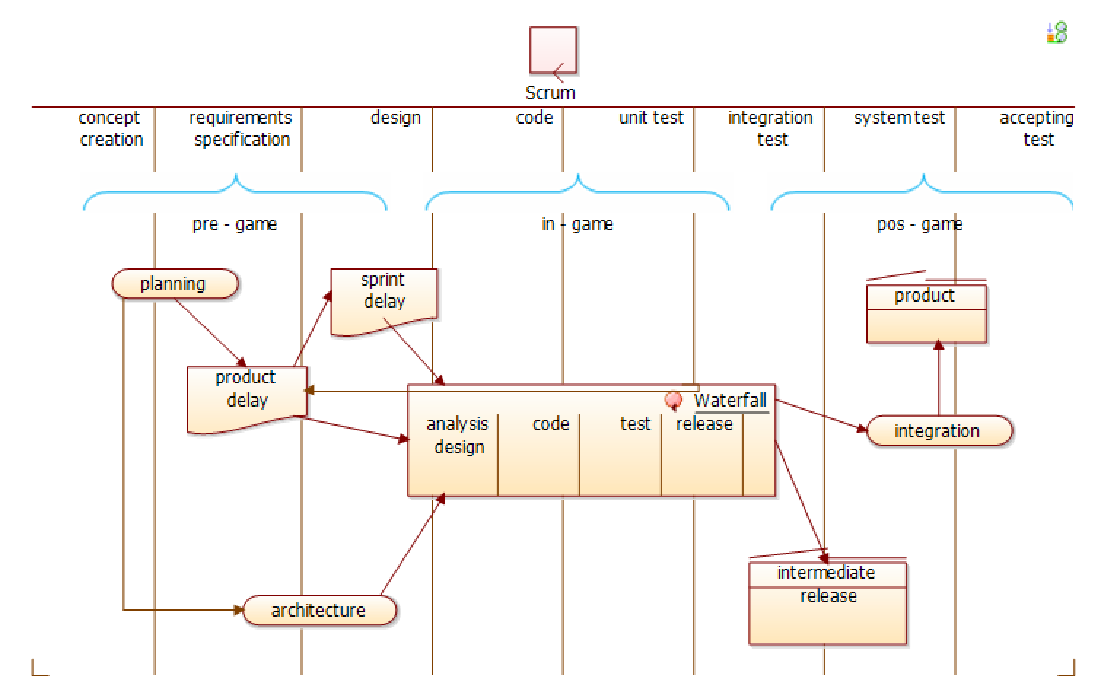
\includegraphics[scale=0.65,]{imagenes/Metodologia/Scrum.pdf}
	\caption{Metodología Scrum.}
	\label{fig:cronograma}
\end{figure}

Haciendo énfasis en todo lo que conlleva hacer uso de esta metodología para el desarrollo de nuestro proyecto, de debe hablar de que se realizará en cada una de las etapas planteadas en esta metodología, también se mostrará el cronograma relacionado con esta metodología y los procesos a utilizar, pero primero que todo se definirá el Scrum Master y Team Members.\\

Scrum Master: la persona encargada de cumplir las tareas de un Scrum Master será Andres Restrepo, dado que por sus cualidades califica perfectamente para llevar a cabo este cargo, además tiene un perfil de un líder dado que supervisará, verificará y será el facilitador del equipo de trabajo.\\

Team members: las personas que conformarán el Team Members serán Daniel Casas, Brayan Esguerra, Andres Restrepo Que tendrán la tarea enfocada hacia el desarrollo del software y los cuales tienen las capacidades técnicas para poder desarrollar el producto a cabalidad.\\

Planeación del Sprint: En este proceso el Scrum Master y el Team Members  se reunirán para planear las actividad o actividades que se encuentran inmersas dentro del sprint a realizar es decir se deben dar prioridad dentro de estas actividades y dar todas la información pertinente como lo es el tiempo existente para esta iteración para poder tener referencias para el próximo sprint.\\

Reunión diaria de Scrum: En cuanto a las reuniones diarias en este proyecto cambiaremos un poco ese concepto dado que aunque se realizarán diariamente, no al inicio del día, sino que por el contrario se hará una reunión finalizando el día para saber que los miembros que participan en estas reuniones puedan hacer y responder preguntas como ¿Qué se hizo durante el día?, ¿Qué se planea hacer el día siguiente? Y saber si se ha presentado algún tipo de inconveniente en el proceso de alcanzar el objetivo además estas reuniones tendrán un intervalo de durabilidad de entre unos 15 a 20 minutos diarios.\\

Revisión del sprint: Cada vez que se dé por terminado un sprint se debe mostrar lo que el equipo ha logrado, es decir un producto terminado referente a ese sprint que se estaba trabajando para saber si esta óptimo o si se deben hacer algunas correcciones esto se analizará dentro del grupo de trabajo y el dueño del producto, aclarando que los sprints serán realizados con las características de el proceso en Cascada.

\section{Scrum - Cascada - Codificación y Reparación}

\subsection{Pre-Game}
En esta sección se  especificará que se hará durante las dos fases que la componen como lo son la planeación y la escenificación.

\subsubsection{Planeación (Planning)}
Durante este segmento o fase se realiza una reunión entre todos los entes involucrados en el desarrollo de este proyecto como lo son the power owner, scrum master y team members  para poder definir la visión, la expectativas y el presupuesto con el que se cuenta para el desarrollo de este además de esto the power owner debe de lanzar la pila de producto que contengan los elementos suficientes para poder entrar a un primer sprint.

\subsubsection{Staging (Escenificación)}
Durante esta fase se tomara en cuenta lo especificado o planteado en la fase anterior es decir en la fase de planeación dado que se tiene que tener claro el presupuesto y los requisitos planteados, es importante traer de la fase de planeación la lista de producto dado que por medio de esta se llegará al planteamiento de los requerimientos los cuales son de suma importancia para el desarrollo de nuestro proyecto. En esta fase se verán involucrado tanto el Scrum Master como el Team Members dado que entre ellos se analizará la lista de producto para poder llegar a unos requerimientos que satisfagan el proyecto.

\subsection{In-Game}
En esta sección se  especifica la duración de cada uno de los sprints por medio de el procesos cascada a el cual se le ha integrado el proceso de codificación y reparación.
\subsubsection{Proceso en Cascada (Waterfall)}
\begin{figure}[H]
	\centering
	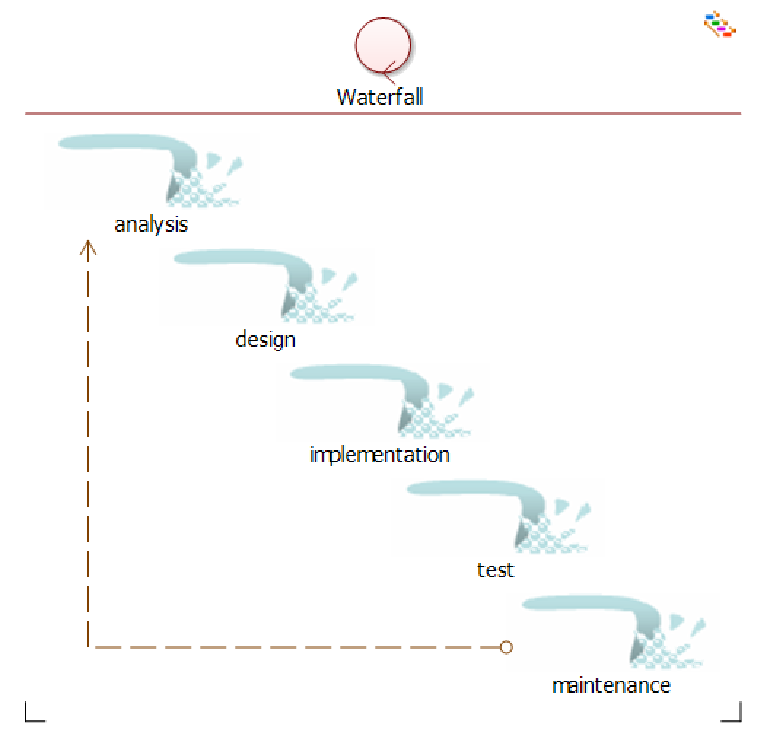
\includegraphics[scale=0.7,]{imagenes/Metodologia/Waterfall.pdf}
	\caption{Proceso Waterfall}
	\label{fig:cronograma}
\end{figure}

\paragraph{Análisis (Analysis)}
Durante esta etapa se tendrán en cuenta los requisitos del sistema planteados por el cliente. Además de esto una parte importante de esta etapa hace referencia al desarrollo de cada uno de los requerimientos, es decir que a través de la información suministrada por el cliente se plantearán cada uno de los requerimientos y se desarrollará la interacción, es decir los casos de uso, casos de secuencia, casos de comunicación y workflow, para así tener planteamientos específicos, concretos y sin lugar a ambigüedades.

\paragraph{Diseño (Design)}
Luego de finalizada la etapa de análisis se tomarán los desarrollos realizados en requerimientos e interacciones, ya que por medio de ellos se planteará un diseño que le brinde solución a la situación problema planteada por el cliente, es así como se tomará cada uno de los requerimientos y se les aplicará este mismo proceso de diseño y solución para poder pasar a la siguiente etapa la cual es la de implementación y poder facilitar este proceso por medio de un diseño claro y conciso.

\paragraph{Implementación (Implementation)}
En esta etapa se hará uso de un nuevo proceso el cual es CODIFICACIÓN Y REPARACIÓN con el cual se busca utilizar cada uno de los diseños o soluciones planteadas y por medio de algoritmia o codificación poder plasmar estas soluciones a nivel de código.

\subparagraph{Codificación y Reparación}
Se utilizará el proceso de codificación y reparación dado que es un modelo simple que está orientado a la parte de desarrollo, pues que encaja perfectamente dentro de la etapa de implementación dentro de la cual se encuentra inmersa, a pesar de que no está compuesta por una etapa de prueba, y es un buen complemento para el correcto y efectivo desarrollo de la codificación.
%imageeeeeeeeeeeeeeeeeeeeeen
\begin{figure}[H]
	\centering
	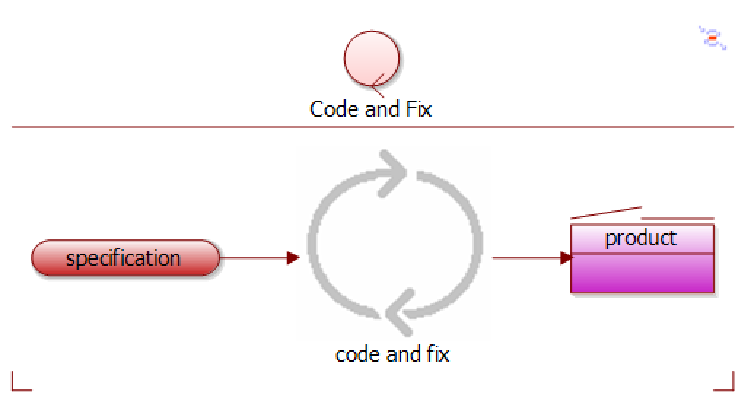
\includegraphics[scale=0.9,]{imagenes/Metodologia/Code-and-fix}
	\caption{Proceso Code and Fix}
	\label{fig:cronograma}
\end{figure}

\subsubparagraph{Especificación}
En esta etapa se hará uso de los requerimientos y los diseños planteados en la etapa de análisis y diseño del proceso en cascada los cuales se analizarán para poder seguir adelante en este proceso y llevar esto a la siguiente etapa la cual es Codificación y Reparación.

\subsubparagraph{Codificación y Reparación}
Durante esta etapa se realizan constantemente ciclos en los cuales se hará uso de esa especificación ya realizada anteriormente para poder tomar cada diseño o solución planteada y así poder traducir esto a un lenguaje que la maquina entienda.

\subsubparagraph{Producto}
Después de dar como finalizada la etapa anterior en esta fase se tendrá el producto final, el cual en este caso será la implementación de un diseño y una solución en particular para que de esta manera sea posible abarcar en su totalidad todas los diseños de  las soluciones planteadas.

\paragraph{Prueba (Test)}
Luego del desarrollo de las soluciones de diseño y su implementación se realizaran pruebas necesarias para poder verificar que nuestro producto final tenga la calidad necesaria para que la cantidad de errores sea mínima con el objetivo de reducir el tiempo de trabajo en la etapa de mantenimiento, además de esto se harán uso de ciertas pruebas como lo son:

Prueba unitaria.
Prueba de integración.
Pruebas del sistema.
Prueba de aceptación.

\paragraph{Mantenimiento (Maintenance)}
En este caso enfocaremos esta etapa a la corrección de los errores encontrados en el producto final, en un dado caso que en la etapa anterior se presente algún tipo de error, se manejará un mantenimiento preventivo y perfectivo dado que por medio este se busca prever posibles errores a futuro direccionándonos a obtener un producto de una muy buena calidad que satisfaga las necesidades del cliente propuestas en la etapa de análisis con un mínimo de requisitos de hardware.


\subsection{Post-Game}
En esta sección se  especificarán las partes que componen esta fase como lo es el release o liberación.

\subsubsection{Release (Liberación)}
En esta etapa se busca dar y entregar el producto final utilizando conjuntamente el concepto de integración, dado que se utilizara para poder unir los subsistemas creados en el in-game y por medio de este término poder integrarlos y unirlos para tener un producto final integrado y finalizado cumpliendo exitosamente lo propuesto al inicio de nuestro proyecto.


\section{Cronograma}
Cabe resaltar que el cronograma planteado está directamente relacionado con nuestro desarrollo de software el cual incluye la metodología Scrum y los procesos en Cascada y, codificación y reparación.

%%%imageeeeen cronograma
%\includegraphics{imagenes/imgs/cronograma}
\begin{figure}[H]
	\centering
	\includegraphics[scale=0.10,]{imagenes/Metodologia/cronograma.pdf}
	\caption{Cronograma de metodología Scrum }
	\label{fig:cronograma}
\end{figure}

\subsection{Pre-Game}
Esta fase tiene una duración de 13 días, en los cuales se buscara cumplir cada una de las funciones que tienen cada una de las etapas que componen el pre-game estos días están distribuidos de la siguiente forma:
\begin{itemize}
	\item \textbf{Planificación}: esta etapa abarca un total de 5 días en los cuales se buscara cumplir la meta propuesta anteriormente.
	\item \textbf{Escenificación}: esta etapa cuenta con  un total de 7 días en los cuales se buscara cumplir las tareas propuestas anteriormente.
	
\end{itemize}

Dentro de esta fase podemos encontrar un primer sprint el cual se desarrollara durante la etapa de escenificación.

\subsection{In-Game}
Esta fase tiene una duración de 60 días en los cuales se buscara cumplir cada una de las funciones que tienen cada una de las etapas que componen el pre-game y estos días están distribuidos de la siguiente forma con el uso de los procesos mencionados anteriormente:

\subsubsection{Cascada}
\begin{itemize}
	\item \textbf{Análisis}: esta etapa cuenta con  un total de 10 días en los cuales se buscará cumplir y analizar lo propuesto en la escenificación y la codificación.
	\item \textbf{Diseño}: esta etapa abarca un total de 30 días en los cuales se buscará cumplir con los diseños de software.
	\item \textbf{Implementación}: esta etapa abarca un total de 18 días en los cuales se usará el proceso de Codificación y Reparacion para llevar acabo el desarrollo de esta.
	\item \textbf{Prueba}: esta etapa no cuenta con días en el calendario dado que no se llegará a esta.
	\item \textbf{Mantenimiento}: al igual que en la etapa de prueba, no se realizará dado que no se llegará a ese punto.
	
	
	
	
\end{itemize}

Dentro de esta fase encontramos 3 sprints de tipo macro ubicado en cada una de la etapas como lo son las rápidas cascadas que se realizaran y cada uno de esos macro-sprint se componen por varios micro-sprint los cuales son el proceso de Codificación y Reparación, esto está relacionado con el número de requerimientos los cuales se pondrán a ser procesados en cada una de estas etapas.

\subsection{Post-Game}
Esta fase tiene una duración de 6 días en los cuales se buscará cumplir cada una de las funciones que tiene la liberación:
\begin{itemize}
	\item \textbf{Liberación}: esta etapa cuenta con un total de 6 días en los cuales se entregará el producto.
\end{itemize}
	


	
	\part{Arquitecura}
	\chapter{Organizacion}

\begin{figure}[h]
	\centering
	\includegraphics[scale=0.5]{imagenes/logoTWP}
	\caption{Two Wheels Parking}
	\label{fig:logotwp}
\end{figure}


\section{Misión}
En Two Wheels Parking ofrecemos soluciones de aparcamiento para bicicletas en la ciudad de Bogotá, ofreciendo una experiencia de tranquilidad, seguridad y organización a nuestros clientes,  buscando incentivar el uso de este medio de transporte como una alternativa limpia y segura.\\

\section{Visión}
Queremos estar comprometidos con los problemas de nuestros clientes de forma transparente y eficaz, convirtiéndonos en un socio de confianza. En Two Wheels Parking queremos ser un referente como una empresa líder en soluciones de aparcamiento, dando a conocer nuestra marca como una empresa ética, responsable y solidaria con nuestros clientes.\\

\section{Estructura Organizacional}
\begin{figure}[h]
	\centering
	\includegraphics[width=1\linewidth]{imagenes/organigrama}
	\caption{Organigrama General de Two Wheels Paking.}
	\label{fig:organigrama}
\end{figure}

\section{Funciones de Negocio y Manual de funciones}

\subsection {Recursos humanos}
\begin{itemize}
	\item Trabajadora social: Profesional encargado del desarrollo de vínculos humanos saludables y buenas relaciones sociales entre los individuos que laboran al interior de la empresa.\\
\end{itemize}

\subsection {Gerencia}
\begin{itemize}
	\item Presidente: Representante, líder y supervisor en la toma de decisiones que guían el rumbo de la compañía. \\
	\item Secretaria: Principal colaboradora del presidente en el área administrativa, dentro de su rol es la encargada de la gestión de la documentación empresarial y de la atención al público.\\
\end{itemize}

\subsection{Seguridad} 
\begin{itemize}
	\item Guardia de seguridad: personal competente para realizar  actividades  de  vigilancia,  inspección,  prevención  y  detección  de  anormalidades  al interior de la Institución.
\end{itemize}

\subsection{Tesorería} 
\begin{itemize}
	\item Tesorero: Encargado de gestionar y dirigir los asuntos relacionados con movimientos económicos o flujos monetarios, tanto captación como desembolsos dentro de la empresa.
\end{itemize}

\subsection{Administrativo y contable} 
\begin{itemize}
	\item Contador Público: Profesional encargado de realizar y verificar los registros contables, tributarios y financieros de la empresa, generando los informes y documentos legales exigidos por la legislación nacional.
	\item Administrador: Responsable de la gestión de recursos materiales y financieros dedicados a la realización y control de las distintas actividades tanto técnica como administrativas mediante una correcta planificación, coordinación y ejecución.
\end{itemize}

\subsection{Ventas y mercadotecnia}
\begin{itemize}
	\item Agentes de ventas: Profesionales capaces de captar y aumentar el número y la calidad de clientes a los cuales la empresa busca prestar una serie de soluciones.
	\item Publicista: Experto en supervisar, coordinar y ejecutar estrategias de publicidad y posicionamiento de imagen tanto de la empresa como de los productos que se generan al interior de ella.
\end{itemize}


\section{Procesos de Negocio}
\begin{figure}[h]
	\centering
	\includegraphics[width=0.8\textwidth]{imagenes/mapProcTWP}
	\caption{Mapa de Procesos de Two Wheels Paking.}
	\label{fig:awesome_image}
\end{figure}

\section{Objetivos}
\subsection{Organizacionales}
\begin{itemize}
	\item Alcanzar un amplio mercado a nivel nacional convirtiéndonos en una de las empresas pioneras de soluciones en colaboración con el medio ambiente, brindando soluciones de parqueo a aquellas personas que hacen uso de un transporte ecológico, esto con el fin de fomentar el uso de dicho transporte y contribuir al desarrollo sustentable.
\end{itemize}

\subsection{Operacionales}
\begin{itemize}
	\item Brindar la mejor calidad de servicio a nuestros clientes, mediante un equipo de trabajo altamente capacitado, convirtiéndonos en una de las empresas distritales con uno de los mejores “Goodwill”.
\end{itemize}

\subsection{Misionales}
\begin{itemize}
	\item Enfocar todos nuestros procesos al uso eficiente de los insumos y recursos, esto mediante el fomento de responsabilidad social tanto al interior como al exterior de la empresa en nuestros empleados, generando así un Impacto ambiental positivo a partir de la producción de nuestros productos y servicios.
\end{itemize}

\subsection{Estratégicos}
\begin{itemize}
	\item Posicionar a la empresa y su marca Two Wheels como una franquicia respetable de parqueo, esto mediante la estandarización y normalización de nuestros procesos, estableciendonos y generando un impacto primeramente a nivel distrital y posteriormente nacional.
\end{itemize}

\section{Valores Organizacionales}
\subsection{Amabilidad:}  En Two Wheels queremos prestar un servicio de calidad al cliente, por lo cual contamos con un equipo de trabajo capacitado el cual atenderá sus inquietudes y propuestas de la mejor manera.
\subsection{Cumplimiento:}
Sabemos que el tiempo y el dinero son recursos importantes, por eso en Two Wheels nos regimos bajo estrictos estándares y políticas internas para que las actividades estipulados se lleven a cabo en los tiempos predefinidos, los que nos convierte en una empresa sólida y seria de cara a nuestros clientes.
\subsection{Seguridad:}
En Two Wheels nos comprometemos con nuestros usuarios para brindar un ambiente seguro para sus vehículos mediante un control de acceso de usuarios efectivo e instalaciones que cuenten con una infraestructura adecuada para proteger a cada usuario y su vehículo.
\subsection{Respeto:}
En Two Wheels creemos que el pilar de toda organización es el respeto mutuo. Por eso, nuestro equipo está enfocado en brindar el mejor servicio a todos nuestros clientes, sin ninguna excepción.
\subsection{Honestidad:}
Como parte de nuestra misión, en Two Wheels creemos en el manejo transparente de nuestros procesos, ofreciendo a nuestros clientes un servicio en el cual puedan confiar.


	\chapter{Achimate -ADM}

El método ADM y en general el marco TOGAF realiza el análisis arquitectónico con alto nivel de abstracción para visualizar, detectar y
	documentar oportunidades y riesgos durante el desarrollo de la arquitectura, direccionando la arquitectura empresarial con la ayuda de sus herramientas.
TOGAF esta compuesto por 3 partes principales el método de desarrollo ADM (Architecture Development Method), la taxonomía empresarial (Enterprise Continuum) y la base de recursos (Architecture Repository). Aborda el desarrollo a partir de 4 niveles de abstracción:
\begin{itemize}
	\item Arquitectura de Negocio
	\item Arquitectura de Aplicación
	\item Arquitectura de Datos
	\item Arquitectura Tecnológica
\end{itemize}
ADM muestra estos niveles de abstracción en diferentes fases que determinan la linea base (baseline) y el final del nivel de abstracción (target), donde el analisis de brecha (figura 4.1) permite conocer el estado final de la arquitectura despues de una o varias iteraciones.
\begin{figure}[h]
	\centering
	\includegraphics[width=0.5\textwidth]{imagenes/Captura.PNG}
	\caption{Analisis de Brecha -Iteraciones ADM}
	\label{fig:gap_analysis}
\end{figure}

Este análisis mide los objetivos de arquitectura y el grado de la madurez alcanzados por la organización.

ADM consta de 8  niveles o etapas y un paso preliminar donde se describen las actividades iniciales, principios y capacidades de la arquitectura objetivo, también se realiza una adaptación del marco de trabajo para ajustarlo a las necesidades de la organización.
\cite{FGuti}

\begin{figure}[h]
	\centering
	\includegraphics[width=0.4\textwidth]{imagenes/Captura1.PNG}
	\caption{Etapas del Método ADM}
	\label{fig:gap_analysis}
\end{figure}

Las primeras cuatro fases definen los niveles de abstracción antes mencionados para el desarrollo de la arquitectura, la fase E de la interacción define oportunidades y soluciones que se deben implementar.

Estas oportunidades y soluciones se identifican e incluyen en el plan de migración, fase F. En esta fase se desarrolla el producto de software con los requerimientos y especificaciones obtenidos de las anteriores fases, luego lleva a su implementación (fase G) y como finalidad lleva la arquitectura de un estado base (baseline) al estado objetivo (target), estas dos fases dan gobernabilidad y gestión de control de cambios a la arquitectura. Este ciclo se repite hasta llegar a la vision establecida en la fase preliminar junto con la vision inicialmente concebida.


\section{TOGAF}
\subsection{Resumen: capa de negocio}

\begin{center}
	\begin{longtable}{|p{5cm}|p{6cm}|p{3cm}|}
		\hline
		\textbf{Concepto} &  \centering \textbf{Definición} & \textbf{Notación} \\
		\hline
		\endfirsthead
		
		
		\hline
		\textbf{Concepto} &  \centering \textbf{Definición} & \textbf{Notación} \\
		\hline
		\endhead
		
		%inicio contenido tabla 
		
		\centering 
		\textbf{Actor de negocio}\\ 
		\textbf{(Business actor)} 
		& Una entidad organizativa que es capaz de realizar el comportamiento.         & 
		\raisebox{-\totalheight}{\includegraphics[scale=0.36]{imagenes/lenguaje/Bussines/actor}}\\
		\hline         
		
		
		\centering \textbf{Papel del negocio}\\ \textbf{(Business role)} & La responsabilidad de realizar un comportamiento específico, al cual un actor puede ser asignado.&\raisebox{-\totalheight}{\includegraphics[scale=0.36,]{imagenes/lenguaje/Bussines/role}}\\
		\hline
		
		
		\centering \textbf{Colaboración Empresarial}\\ \textbf{(Business Collaboration)} & Un agregado de dos o más funciones empresariales que trabajan juntas para realizar un comportamiento colectivo. &  \raisebox{-\totalheight}{\includegraphics[scale=0.36,] {imagenes/lenguaje/Bussines/collaboration}}\\ 
		\hline
		
		
		\centering \textbf{Interfaz de negocios}\\ \textbf{(Business interface)} & Un punto de acceso donde un servicio comercial está disponible para el medio ambiente..&  \raisebox{-\totalheight}{\includegraphics[scale=0.36,]{imagenes/lenguaje/Bussines/interface}}\\ 
		\hline
		
		\centering \textbf{Ubicación}\\ \textbf{(Location)}& Un punto conceptual o extensión en el espacio.&  
		\raisebox{-\totalheight}{\includegraphics[scale=0.36,]{imagenes/lenguaje/Bussines/location}}\\ 
		\hline
		
		\centering \textbf{Objeto de negocio}\\ \textbf{(Business Object)}& Un elemento pasivo que tiene relevancia desde una perspectiva empresarial.&  
		\raisebox{-\totalheight}{\includegraphics[scale=0.36,]{imagenes/lenguaje/Bussines/object}}\\ 
		\hline
		
		\centering \textbf{Proceso de negocio}\\ \textbf{(Business Process)}& Un elemento de comportamiento que agrupa el comportamiento basado en un ordenamiento de actividades. Se pretende producir un conjunto definido de productos o servicios empresariales.&  
		\raisebox{-\totalheight}{\includegraphics[scale=0.36,]{imagenes/lenguaje/Bussines/process}}\\ 
		\hline
		
		\centering \textbf{Función de negocio}\\ \textbf{(Business Function)}& Un elemento de comportamiento que agrupa el comportamiento basado en un conjunto seleccionado de criterios (normalmente requeridos por los recursos empresariales y / o las competencias).&  
		\raisebox{-\totalheight}{\includegraphics[scale=0.36,]{imagenes/lenguaje/Bussines/funtion}}\\ 
		\hline
		
		\centering \textbf{Interacción de negocios}\\ \textbf{(Business Interaction)}& Un elemento de comportamiento que describe el comportamiento de una colaboración comercial.&  
		\raisebox{-\totalheight}{\includegraphics[scale=0.36,]{imagenes/lenguaje/Bussines/interaction}}\\ 
		\hline
		
		\centering \textbf{Evento de negocios}\\ \textbf{(Business Event)}& Algo que sucede (internamente o externamente) e influye en el comportamiento.&  
		\raisebox{-\totalheight}{\includegraphics[scale=0.36,]{imagenes/lenguaje/Bussines/event}}\\ 
		\hline
		
		\centering \textbf{Servicio de negocio o empresarial}\\ \textbf{(Business Service)}& Un servicio que satisface una necesidad de negocio para un cliente (interno o externo a la organización).&  
		\raisebox{-\totalheight}{\includegraphics[scale=0.36,]{imagenes/lenguaje/Bussines/service}}\\ 
		\hline
		
		\centering \textbf{Representación}\\ \textbf{(Representation)}& Una forma perceptible de la información transportada por un objeto de negocio.&  
		\raisebox{-\totalheight}{\includegraphics[scale=0.36,]{imagenes/lenguaje/Bussines/representation}}\\ 
		\hline
		
		\centering \textbf{Significado}\\ \textbf{(Meaning)}& Los conocimientos o experiencia presentes en un objeto de negocio o su representación, dado un contexto particular.&  
		\raisebox{-\totalheight}{\includegraphics[scale=0.36,]{imagenes/lenguaje/Bussines/meaning}}\\ 
		\hline
		
		\centering \textbf{Valor}\\ \textbf{(Value)}& El valor relativo, la utilidad o la importancia de un servicio o producto comercial.&  
		\raisebox{-\totalheight}{\includegraphics[scale=0.36,]{imagenes/lenguaje/Bussines/value}}\\ 
		\hline
		
		
		\centering \textbf{Producto}\\ \textbf{(Product)}& Un conjunto coherente de servicios, acompañado de un contrato / conjunto de acuerdos, que se ofrece en su conjunto a clientes (internos o externos).&  
		\raisebox{-\totalheight}{\includegraphics[scale=0.36,]{imagenes/lenguaje/Bussines/product}}\\ 
		\hline
		
		
		\centering \textbf{Contrato}\\ \textbf{(Contract)}& Una especificación formal o informal de acuerdo que especifica los derechos y obligaciones asociados con un producto.&  
		\raisebox{-\totalheight}{\includegraphics[scale=0.36,]{imagenes/lenguaje/Bussines/contract}}\\ 
		\hline
		
		\caption{Capa de Negocio}
		\label{capa-business}
	\end{longtable}
\end{center}

\subsection{Resumen: capa de aplicación}
\begin{center}
\begin{longtable}{| >{\centering\arraybackslash}m{3cm} | >{\arraybackslash}m{6cm} | p{4cm} | p{5cm} | p{4cm} |}
	
		\hline
		\textbf{Concepto} &  \centering \textbf{Definición} & \textbf{Notación} \\
		\hline
		\endfirsthead
		
		
		\hline
		\textbf{Concepto} &  \centering \textbf{Definición} & \textbf{Notación} \\
		\hline
		\endhead
		
		Componente de Aplicación & 
		\vspace{1mm} Una parte modular, desplegable y reemplazable de un sistema de software que encapsula su comportamiento y datos y los expone a través de un conjunto de interfaces. & 
		\includegraphics[width=35mm,trim=0 0 0 -2mm]{imagenes/lenguaje/Aplication/componentApp}\\ 
		\hline
		
		Colaboración de Aplicación & 
		\vspace{1mm} 
		 Un agregado de dos o más componentes de aplicación que trabajan juntos para realizar un comportamiento colectivo.& 
		\includegraphics[width=35mm,trim=0 0 0 -6mm]{imagenes/lenguaje/Aplication/collaborationApp}\\ 
		\hline
		
		Interfaz de Aplicación &
		\vspace{1mm} Un punto de acceso donde un servicio de aplicación está disponible para un usuario u otro componente de aplicación &  
		\includegraphics[width=35mm,trim=0 0 0 -2mm]{imagenes/lenguaje/Aplication/interfaceApp}\\ 
		\hline
				
		Objeto de Datos &
		\vspace{1mm} Un elemento pasivo adecuado para el procesamiento automatizado.& 
		\includegraphics[width=15mm,trim=0 0 0 -6mm]{imagenes/lenguaje/Aplication/dataObjectApp}  \\ 
		\hline
		
		Función de Aplicación & 
		\vspace{1mm} Un elemento de comportamiento que agrupa el comportamiento automatizado que puede ser realizado por un componente de aplicación.& 
		\includegraphics[width=35mm,trim=0 0 0 -6mm]{imagenes/lenguaje/Aplication/functionApp}  \\ 
		\hline 
		
		Interacción de Aplicación &
		\vspace{1mm} Un elemento de comportamiento que describe el comportamiento de una colaboración de aplicación& 
		\includegraphics[width=35mm,trim=0 0 0 -6mm]{imagenes/lenguaje/Aplication/interactionApp}  \\ 
		\hline 	
		
		Servicio de Aplicación &
		\vspace{1mm} Un servicio que expone un comportamiento automatizado & 
		\includegraphics[width=25mm,trim=0 0 0 -2mm]{imagenes/lenguaje/Aplication/serviceApp} \\ 
		\hline 

		\caption{Capa de Aplicación}
		\label{capa-aplicacion}
\end{longtable}
\end{center}



\subsection{Resumen: capa de motivación}
\begin{center}
\begin{longtable}{| >{\centering\arraybackslash}m{3cm} | >{\arraybackslash}m{6cm} | p{4cm} | p{5cm} | p{4cm} |}
	
		\hline
		\textbf{Concepto} &  \centering \textbf{Definición} & \textbf{Notación} \\
		\hline
		\endfirsthead
		
		
		\hline
		\textbf{Concepto} &  \centering \textbf{Definición} & \textbf{Notación} \\
		\hline
		\endhead
		
		Interesados & 
		\vspace{1mm} El rol de un individuo, equipo u organización (o clases de ellos) que representa sus intereses o preocupaciones, relativas al resultado de la arquitectura.& 
		\includegraphics[width=25mm,trim=0 0 0 -20mm]{imagenes/lenguaje/Motivational/stakeholder}\\ 
		\hline
		
		Conductor & 
		\vspace{1mm} 
		 Algo que crea, motiva y alimenta el cambio en una organización. & 
		\includegraphics[width=25mm,trim=0 0 0 -8mm]{imagenes/lenguaje/Motivational/driver}\\ 
		\hline
		
		Evaluación &
		\vspace{1mm} El resultado de algunas evaluaciones de algunos conductores. & 
		\includegraphics[width=25mm,trim=0 0 0 -8mm]{imagenes/lenguaje/Motivational/assessment}\\ 
		\hline
		
		Objetivo & 
		\vspace{1mm} Un estado final que una parte interesada desea lograr.& 
		\includegraphics[width=25mm,trim=0 0 0 -8mm]{imagenes/lenguaje/Motivational/goal}  \\ 
		\hline
		
		Requerimineto &
		\vspace{1mm} Una declaración de necesidad que debe ser realizada por un sistema. & 
		\includegraphics[width=35mm,trim=0 0 0 -8mm]{imagenes/lenguaje/Motivational/requirement}  \\ 
		\hline
		
		Restricción & 
		\vspace{1mm} Una restricción de la forma en que se realiza un sistema.& 
		\includegraphics[width=35mm,trim=0 0 0 -8mm]{imagenes/lenguaje/Motivational/constraint}  \\ 
		\hline 
		
		Principio &
		\vspace{1mm} Una propiedad normativa de todos los sistemas en un contexto dado, o la forma en que se realizan.& 
		\includegraphics[width=25mm,trim=0 0 0 -8mm]{imagenes/lenguaje/Motivational/principle}  \\ 
		\hline 	
		
	\caption{Capa de Motivación}
	\label{capaMotivacion}
\end{longtable}
\end{center}


\subsection{Resumen: capa de proyecto}
\begin{center}
\begin{longtable}{| >{\centering\arraybackslash}m{3cm} | >{\arraybackslash}m{6cm} | p{4cm} | p{5cm} | p{4cm} |}
	
		\hline
		\textbf{Concepto} &  \centering \textbf{Definición} & \textbf{Notación} \\
		\hline
		\endfirsthead
		
		
		\hline
		\textbf{Concepto} &  \centering \textbf{Definición} & \textbf{Notación} \\
		\hline
		\endhead
		
		Paquete de Trabajo & 
		\vspace{1mm} Una serie de acciones diseñadas para lograr una meta única dentro de un tiempo especificado.&
		\includegraphics[width=30mm,trim=0 0 0 -8mm]{imagenes/lenguaje/Proyect/WorkPackage.png}\\ 
		\hline
		
		Entregable & 
		\vspace{1mm} 
		 Un resultado definido con precisión de un paquete de trabajo (work package).& 
		\includegraphics[width=25mm,trim=0 0 0 -8mm]{imagenes/lenguaje/Proyect/Deliverable.png}\\ 
		\hline
		
		Meseta &
		\vspace{1mm} Un estado relativamente estable de la arquitectura que existe durante un período de tiempo limitado. &  
		\includegraphics[width=30mm,trim=0 0 0 -8mm]{imagenes/lenguaje/Proyect/Plateau.png}\\ 
		\hline
		
		Brecha & 
		\vspace{1mm} Resultado de un análisis de la brecha entre dos mesetas (plateaus).&  
		\includegraphics[width=25mm,trim=0 0 0 -8mm]{imagenes/lenguaje/Proyect/Gap.png}  \\ 
		\hline
		\caption{Capa de Proyecto}
	\label{capa-proyecto}
\end{longtable}
\end{center}


\subsection{Resumen: capa de tecnologia}
\begin{center}
\begin{longtable}{| >{\centering\arraybackslash}m{3cm} | >{\arraybackslash}m{6cm} | p{4cm} | p{5cm} | p{4cm} |}
	
		\hline
		\textbf{Concepto} &  \centering \textbf{Definición} & \textbf{Notación} \\
		\hline
		\endfirsthead
		
		
		\hline
		\textbf{Concepto} &  \centering \textbf{Definición} & \textbf{Notación} \\
		\hline
		\endhead
		
		Nodo & 
		\vspace{1mm} Un recurso computacional sobre el cual los artefactos pueden ser almacenados o	desplegados para su ejecución.&
		\includegraphics[width=30mm,trim=0 0 0 -2mm]{imagenes/lenguaje/tecnologia/nodo}\\ 
		\hline
		
		Dispositivo & 
		\vspace{1mm} 
		Un recurso de hardware en el que los	artefactos se pueden almacenar o desplegar 	para su ejecución.& 
		\includegraphics[width=35mm,trim=0 0 0 -2mm]{imagenes/lenguaje/tecnologia/dispositivo}\\ 
		\hline
		
		Red &
		\vspace{1mm} Un medio de comunicación entre dos o más dispositivos.& 
		\includegraphics[width=25mm,trim=0 0 0 -2mm]{imagenes/lenguaje/tecnologia/red}\\ 
		\hline
		
		Ruta de Comunicación & 
		\vspace{1mm} Un enlace entre dos o más nodos, a	través del cual estos nodos pueden intercambiar datos.& 
		\includegraphics[width=35mm,trim=0 0 0 -2mm]{imagenes/lenguaje/tecnologia/comunicacion}  \\ 
		\hline
		
		Interfaz de infraestructura &
		\vspace{1mm} Un punto de acceso donde los servicios de infraestructura ofrecidos por un nodo pueden ser accedidos por otros nodos y componentes de la aplicación.&  
		\includegraphics[width=35mm,trim=0 0 0 -2mm]{imagenes/lenguaje/tecnologia/interfaz}  \\ 
		\hline
		
		Software del Sistema & 
		\vspace{1mm} Un entorno de software para tipos específicos de componentes y objetos que	se despliegan en él en forma de artefactos.& 
		\includegraphics[width=35mm,trim=0 0 0 -2mm]{imagenes/lenguaje/tecnologia/software}  \\ 
		\hline 
		
		Función de Infraestructura &
		\vspace{1mm} Un elemento de comportamiento que agrupa el comportamiento de infraestructura que puede ser realizado por un	nodo.& 
		\includegraphics[width=35mm,trim=0 0 0 -2mm]{imagenes/lenguaje/tecnologia/funcion}  \\ 
		\hline 	
		
		Servicio de Infraestructura &
		\vspace{1mm} Una unidad de funcionalidad visible externamente, proporcionada por uno o más nodos, expuesta a través de interfaces bien definidas y significativa para el entorno.		&  
		\includegraphics[width=35mm,trim=0 0 0 -2mm]{imagenes/lenguaje/tecnologia/servicio} \\ 
		\hline 
		
		Artefacto &
		\vspace{1mm} Una pieza física de datos que se utiliza ose produce en un proceso de desarrollo de software, o mediante el despliegue y la operación de un sistema.&
		\includegraphics[width=35mm,trim=0 0 0 -2mm]{imagenes/lenguaje/tecnologia/artefacto}  \\ 
		\hline
		

	\caption{Conceptos de Capa de Tecnología}
	
\end{longtable}
\end{center}


\subsection{Resumen Relaciones}

\subsubsection{Relaciones Estructurales}
\begin{center}
	\begin{longtable}[h]{| >{\centering\arraybackslash}m{3cm} | >{\arraybackslash}m{6cm} | p{4cm} | p{5cm} | p{4cm} |}
		
		\hline
		\textbf{Concepto} &  \centering \textbf{Definición} & \textbf{Notación} \\
		\hline
		\endfirsthead
		
		
		\hline
		\textbf{Concepto} &  \centering \textbf{Definición} & \textbf{Notación} \\
		\hline
		\endhead
		
		Asociacion       
		& \vspace{1mm} La asociación modela una relación entre
		objetos que no están cubiertos por otra más
		relación específica.        
		&\includegraphics[width=30mm,trim=0 0 0 -2mm]{imagenes/lenguaje/relaciones/asociacion}  \\ \hline
		
		Acceso
		& \vspace{1mm} La relación de acceso modela el acceso de
		Conceptos conductuales para negocios o datos
		objetos.            
		& \includegraphics[width=35mm,trim=0 0 0 -2mm]{imagenes/lenguaje/relaciones/acceso}  \\ \hline
		
		Usado por        
		&\vspace{1mm} El utilizado por la relación modela el uso de
		servicios por procesos, funciones o
		interacciones y el acceso a las interfaces por
		roles, componentes o colaboraciones.               
		& \includegraphics[width=25mm,trim=0 0 0 -2mm]{imagenes/lenguaje/relaciones/usadopor}  \\ \hline
		
		Realización	
		& \vspace{1mm} La relación de realización vincula una lógica
		entidad con una entidad más concreta que
		se da cuenta.              
		& \includegraphics[width=35mm,trim=0 0 0 -2mm]{imagenes/lenguaje/relaciones/realizacion}  \\ \hline
		
		Asignación &\vspace{1mm} La relación de asignación vincula unidades de
		comportamiento con elementos activos (por ejemplo, roles,
		componentes) que los realizan, o roles con
		actores que los cumplen. 
		&  \includegraphics[width=35mm,trim=0 0 0 -2mm]{imagenes/lenguaje/relaciones/asignacion}  \\ \hline
		
		Agregacion
		&\vspace{1mm}  La relación de agregación indica que un
		el objeto agrupa varios otros objetos.
		& \includegraphics[width=35mm,trim=0 0 0 -2mm]{imagenes/lenguaje/relaciones/agregacion}  \\ \hline 
		
		Composición 
		&\vspace{1mm} La relación de composición indica que
		un objeto se compone de uno o más
		objetos.
		& \includegraphics[width=35mm,trim=0 0 0 -2mm]{imagenes/lenguaje/relaciones/composicion}  \\ \hline 			
		
		\caption{Conceptos de Capa de Relaciones Estructurales}
		
	\end{longtable}
\end{center}

\subsubsection{Relaciones Dinámicas}
\begin{center}
	\begin{longtable}[h]{| >{\centering\arraybackslash}m{3cm} | >{\arraybackslash}m{6cm} | p{4cm} | p{5cm} | p{4cm} |}
		
		\hline
		\textbf{Concepto} &  \centering \textbf{Definición} & \textbf{Notación} \\
		\hline
		\endfirsthead
		
		
		\hline
		\textbf{Concepto} &  \centering \textbf{Definición} & \textbf{Notación} \\
		\hline
		\endhead
		
		Flujo      
		& \vspace{1mm} La relación de flujo describe el intercambio
		o transferencia de, por ejemplo, información o
		valor entre procesos, función,
		interacciones y eventos.       
		&\includegraphics[width=30mm,trim=0 0 0 -2mm]{imagenes/lenguaje/relaciones/flujo}  \\ \hline
		
		Desencadenante
		& \vspace{1mm} La relación de activación describe el
		relaciones temporales o causales entre
		procesos, funciones, interacciones y eventos.  
		& \includegraphics[width=35mm,trim=0 0 0 -2mm]{imagenes/lenguaje/relaciones/triggering}  \\ \hline
		
		\caption{Conceptos de Capa de Relaciones Dinámicas}
		
	\end{longtable}
\end{center}

\subsubsection{Otras Relaciones}
\begin{center}
	\begin{longtable}[h]{| >{\centering\arraybackslash}m{3cm} | >{\arraybackslash}m{6cm} | p{4cm} | p{5cm} | p{4cm} |}
		
		\hline
		\textbf{Concepto} &  \centering \textbf{Definición} & \textbf{Notación} \\
		\hline
		\endfirsthead
		
		
		\hline
		\textbf{Concepto} &  \centering \textbf{Definición} & \textbf{Notación} \\
		\hline
		\endhead
		
		Agrupamiento     
		& \vspace{1mm} La relación de agrupamiento indica que
		objetos del mismo tipo o tipos diferentes
		pertenecen juntos basados en algunos
		característica.   
		&\includegraphics[width=15mm,trim=0 0 0 -2mm]{imagenes/lenguaje/relaciones/agrupacion}  \\ \hline
		
		Union
		& \vspace{1mm} Un cruce se usa para conectar relaciones de
		el mismo tipo
		& \includegraphics[width=10mm,trim=0 0 0 -2mm]{imagenes/lenguaje/relaciones/union}  \\ \hline
		
		
		
		Especialización
		& \vspace{1mm}La relación de especialización indica que
		un objeto es una especialización de otro objeto.
		& \includegraphics[width=35mm,trim=0 0 0 -2mm]{imagenes/lenguaje/relaciones/especializacion}  \\ \hline
		
		
		\caption{Conceptos de Capa de Relaciones Dinámicas}
		
	\end{longtable}
\end{center}

	\chapter{Negocio}

\section{Introducción}
En esta capa se busca dar información acerca de una serie  de conceptos informativos para dar relevancia  en el dominio empresarial: un producto y contrato asociado, el significado de los objetos de negocio y el valor de los productos y servicios empresariales.\\
Para ello es necesario el diseño de 6 puntos de vista dentro de los cuales se encuentran: de organización, de cooperación de actor, de función de negocio, de proceso de negocio, de cooperación de proceso de negocio y de producto.\\
Los puntos de vista se mostrarán en dos partes, la primera de ellas será el modelo donde se encontrará una descripción del punto de vista acompañado de una tabla con la información de este y el meta-modelo correspondiente, en la segunda parte se encontrará el caso de estudio, es decir, el modelo donde será aplicado el meta-modelo previamente visto al proyecto y la organización en la que se está trabajando.
\newpage

\section{Punto de Vista de Organización}
\subsection{Descripción}
El punto de vista organizacional en la organización de la compañía, departamento, red de compañías, u otra identidad organizacional. Esto es posible para presentar modelos en este punto de vista como diagramas de bloques anidados, pero en el camino mas tradicional, tal como mapas organizacionales. El punto de vista organizacional es muy tratado en 	la identificación de competencias, autoridades y responsables en la organización.

\subsubsection{Metamodelo}
\begin{figure}[h]
	\centering
	\includegraphics[width=0.7\textwidth]{imagenes/Metamodelos/Negocio/meta_organizacion.PDF}
	\caption{Metamodelo: Punto de Vista de Organización}
	\label{fig:gap_analysis}
\end{figure}

\subsubsection{Caso de Estudio}
En el siguiente punto de vista podemos resaltar la sucursal como localización principal de la organización; adicionalmente, se puede observar la participación de actores quienes son los pilares fundamentales para la realización de los principales procesos en la compañía. Estos son: Seguridad y Administración.

\begin{figure}[h]
	\centering
	\includegraphics[width=0.3\textwidth]{imagenes/Caso_estudio/Negocio/Organizacion.PDF}
	\caption{Caso de estudio: Punto de Vista de Organización}
	\label{fig:gap_analysis}
\end{figure}




\section{Punto de Vista de Cooperación de Actor}
\subsection{Descripción}
El punto de vista de Cooperación de actor se enfoca en las relaciones que se presentan entre un actor y su entorno, se puede decir que es un diagrama de contexto en el cual se coloca la organización en su entorno, además de esto se puede evidenciar clientes, proveedores y compañeros de negocio, tiene como objetivo determinar dependencias y colaboraciones externas y ver la relación con los actores que se encuentran en este diagrama, tenemos por otra parte que en este punto de vista se puede evidenciar el número de actores cooperantes  de negocio van a tener participación en esta capa o cuantos componentes de aplicación interactúan para formar un proceso de negocio.

\subsubsection{Metamodelo}
\begin{figure}[h]
	\centering
	\includegraphics[width=0.7\textwidth]{imagenes/Metamodelos/Negocio/meta_cooperacion_actor.png}
	\caption{Metamodelo: Punto de Vista de Organización}
	\label{fig:gap_analysis}
\end{figure}




\subsubsection{Caso de Estudio}
La colaboración Espacio de Parqueadero, surge de la interacción de los roles Sucursal y Clientes del Parqueadero. Por parte de la sucursal, brindando el terrero de parqueo; y por parte de los clientes, al realizar el uso del mismo a través de la interface que se encuentra de cara a ellos, la Recepción.
\begin{figure}[h]
	\centering
	\includegraphics[width=1.0\textwidth]{imagenes/Caso_estudio/Negocio/CopActor.PDF}
	\caption{Caso de estudio: Punto de Vista de Cooperación de Actor}
	\label{fig:gap_analysis}
\end{figure}










\section{Punto de Vista de Función de Negocio}
\subsection{Descripción}
El punto de vista Función de negocio muestra las principales funciones de negocio de una organización y sus relaciones en términos de los flujos de información, valor o bienes entre ellos. Las funciones empresariales se utilizan para representar los aspectos más estables de una empresa en términos de las actividades primarias que realiza, independientemente de los cambios organizacionales o desarrollos tecnológicos.

Por lo tanto, la arquitectura de la función comercial de las empresas que operan en el mismo mercado a menudo muestran similitudes cercanas. Por lo tanto, el punto de vista de la función empresarial proporciona una visión de alto nivel de las operaciones generales de la empresa y puede utilizarse para identificar las competencias necesarias o estructurar una organización de acuerdo con sus principales actividades.


\subsubsection{Metamodelo}
\begin{figure}[h]
	\centering
	\includegraphics[width=0.6\textwidth]{imagenes/Metamodelos/Negocio/meta_funcion_negocio.png}
	\caption{Metamodelo: Punto de Vista de Función de Negocio}
	\label{fig:gap_analysis}
\end{figure}



\subsubsection{Caso de Estudio}
En el siguiente punto de vista se resalta la presencia de los actores Operario y Jefe de Seguridad, quienes llevan a cabo funciones específicas de los roles de Operación y Seguridad, tales como: Registro de Ingreso, Asignación de Parqueadero, Registro de Usuarios, Registro de Pagos, Registro de Retiros y Verificación de propiedad del vehículo.

\begin{figure}[h]
	\centering
	\includegraphics[width=0.7\textwidth]{imagenes/Caso_estudio/Negocio/FunNegocio.PDF}
	\caption{Caso de estudio: Punto de vista de función de negocio.}
	\label{fig:gap_analysis}
\end{figure}








\section{Punto de Vista de Proceso de Negocio}
\subsection{Descripción}
El punto de vista de proceso de negocio es usado para ver la estructura desde un nivel alto además de esto de poder evidenciar la composición de uno o más procesos de negocio, dentro de este punto de vista podemos resaltar que se enfoca en los servicios que un proceso de negocio puede ofrecer al cliente mostrando como este proceso puede contribuir para la realización de productos, por otro lado se puede hacer una asociación en cuanto a responsabilidades que tienen los actores asociados y los roles dentro de este proceso de negocio y por último en este punto de vista podemos evidenciar la información utilizada por el proceso de negocio.

\subsubsection{Metamodelo}
\begin{figure}[h]
	\centering
	\includegraphics[width=0.6\textwidth]{imagenes/Metamodelos/Negocio/meta_proceso_negocio.png}
	\caption{Metamodelo: Punto de Vista de Proceso de Negocio}
	\label{fig:gap_analysis}
\end{figure}


\subsubsection{Caso de Estudio}
En este punto de vista podemos resaltar el proceso principal de la organización: Renta de espacio de parqueo, el cual es originado por una solicitud del espacio y finaliza en el retiro del vehículo. Dentro de este proceso tenemos los subprocesos de: Registro de Usuario, Registro de Ingreso, Asignación de Espacio, Vigilancia de Vehículo, Cálculo de tarifa y Registro de Pago.

\begin{figure}[h]
	\centering
	\includegraphics[width=1.0\textwidth]{imagenes/Caso_estudio/Negocio/ProNegocio.PDF}
	\caption{Caso de estudio: Punto de vista de proceso de negocio.}
	\label{fig:gap_analysis}
\end{figure}

\section{Punto de vista de Cooperación de procesos de negocio.}
\subsection{Descripción}
El punto de vista de Cooperación de Proceso de Negocio se utiliza para mostrar las relaciones de
uno o más procesos de negocio entre sí y / o con su entorno. Puede utilizarse tanto para crear un diseño
de alto nivel de procesos empresariales dentro de su contexto como para proporcionar un gestor
operativo responsable de uno o más de dichos procesos con información sobre sus dependencias

\subsubsection{Metamodelo}
\begin{figure}[h]
	\centering
	\includegraphics[width=0.6\textwidth]{imagenes/Metamodelos/Negocio/meta_cooperacion_proceso_negocio.png}
	\caption{Metamodelo: Punto de Vista de Cooperación de Negocio}
	\label{fig:gap_analysis}
\end{figure}



\subsubsection{Caso de Estudio}
Adicional al punto de vista anterior, se evidencian los roles involucrados, Administrador y Agente de Seguridad, en el proceso Renta de espacio de parqueo, para llevar a cabo el cumplimiento del servicio fundamental de la organización, Renta de espacio de parqueadero y vigilancia para bicicletas.

\begin{figure}[h]
	\centering
	\includegraphics[width=1.0\textwidth]{imagenes/Caso_estudio/Negocio/CoProNegocios.PDF}
	\caption{Caso de estudio: Punto de vista de colabroacion de procesos de negocio.}
	\label{fig:gap_analysis}
\end{figure}


\section{Punto de Vista de Producto}

\subsection{Descripción}
El punto de vista del producto representa el valor que ese producto ofrece a los clientes u otros involucrados y muestra la composición de uno o mas productos en términos de los servicios constituidos y la asociación de contratos u otros acuerdos. Esto también puede ser usado para mostrar los canales de interfaces que este producto ofrece, y los eventos asociados con el producto. Un punto de vista del producto es típicamente usado en el desarrollo del producto a el diseño del producto por la composición de servicios existentes o la identificación que nuevos servicios tiene que ser creados para este producto,dando el valor a las expectativas del cliente para este. Este puede servir para la entrada para la arquitectura del proceso de negocio y otros que necesiten diseñar el proceso y ICT realizan estos productos. 

\subsubsection{Metamodelo}
\begin{figure}[h]
	\centering
	\includegraphics[width=0.5\textwidth]{imagenes/Metamodelos/Negocio/meta_producto.png}
	\caption{Metamodelo: Punto de Vista de Prodcuto}
	\label{fig:gap_analysis}
\end{figure}


\subsubsection{Caso de Estudio}
El producto principal que ofrece la organización, como se evidencia en los puntos de vista anteriores, es el espacio de parqueo, el cual se caracteriza por proponer espacios adecuados y seguros para las bicicletas de los clientes, a la vez de ofrecer un servicio integral de vigilancia permanente para los vehículos, soportados por sus correspondientes procesos.
\begin{figure}[h]
	\centering
	\includegraphics[width=0.8\textwidth]{imagenes/Caso_estudio/Negocio/Producto.PDF}
	\caption{Caso de estudio: Punto de vista de producto}
	\label{fig:gap_analysis}
\end{figure}



	\chapter{Capa de Aplicación}

\section{Introducción}
En esta capa de aplicaciones observaremos los principales conceptos de comunicación entre componentes por medio de interfaces, donde en los siguientes diagramas se pueden observar los principales comportamientos del aplicativo mediante 4 puntos de vista: Comportamiento de aplicación, Cooperación de aplicación, Estructura de aplicación y el uso de la aplicación.\\
Tal como mencionamos anteriormente, en nuestra capa de aplicación se caracteriza por poseer una arquitectura de componentes, de tal forma que  mostramos las principales funciones dentro de cada componente y ademas como se relacionan y comunican cada uno de estos, de tal forma que observemos como sera el comportamiento y la logica de la aplicación.\\
\\
\\
\\
\\
\\
\\
\\
\\
\\
\\
\\
\\
\\
\\
\\
\section{Punto de Vista de Comportamiento de Aplicación}
\subsection{Descripción}
El punto de vista de comportamiento de aplicación, describe el comportamiento interno de la aplicación, que este realiza uno o más servicios de aplicaciones. El punto de vista es útil en diseñar el principal comportamiento de la aplicación, o identificar superposición funcional entre diferentes aplicación.

\subsubsection{Metamodelo}
\begin{figure}[h]
	\centering
	\includegraphics[width=0.6\textwidth]{imagenes/Metamodelos/Aplicacion/meta_comportamiento_aplicacion.png}
	\caption{Metamodelo: Punto de Vista de Comportamiento de Aplicación.}
	\label{fig:gap_analysis}
\end{figure}

\subsubsection{Caso de Estudio}
En el presente caso de estudio, podemos observar el componente aplicación de la aplicación Two Wheels Digital, el cual se divide compone a su vez de componentes más pequeños como lo son Pagos, que se encarga de cumplir las funciones de cálculo de la tarifa y recepción del pago realizado por cada cliente. Por otra parte, el Gestor de Espacios encargado de la administración de los espacios de parqueo; el Gestor de Usuarios quien lleva a cabo el proceso de registro y validación. Por último, el componente de Estadísticas el cual elabora reportes sobre la renta de los espacios de parqueo.
\begin{figure}[h]
	\centering
	\includegraphics[width=0.7\textwidth]{imagenes/Caso_Estudio/Aplicacion/ComAplicacion.PDF}
	\caption{Caso de estudio: Punto de vista de comportamiento de aplicación.}
	\label{fig:gap_analysis}
\end{figure}




\section{Punto de Vista de Cooperación de Aplicación}
\subsection{Descripción}
El punto de vista Cooperación de aplicación describe las relaciones entre los componentes de la aplicaciones en términos de la información que se maneja entre ellos además de esto también se puede enfocar en términos de los servicios que estos ofrecen y de los que hacen uso. Este punto de vista también es usado para crear una visión general de todo el contexto de aplicación de una organización. Este punto de vista también es usado para expresar la cooperación interna de servicios que trabajando de una forma conjunta soportan la ejecución de un proceso de negocio.

\subsubsection{Metamodelo}
\begin{figure}[h]
	\centering
	\includegraphics[width=0.7\textwidth]{imagenes/Metamodelos/Aplicacion/meta_cooperacion_aplicacion.png}
	\caption{Metamodelo: Punto de Vista de Cooperación de Aplicación.}
	\label{fig:gap_analysis}
\end{figure}

\subsubsection{Caso de Estudio}
Por medio de este punto de vista, se resalta la arquitectura general de tres capas de la aplicación Two Wheels Digital en donde el componente principal de interfaz se encuentra ubicado en la capa de presentación; los componentes Gestor de Usuarios, Gestor de Espacios, Pagos y Estadísticas se ubican en la capa de negocio, y finalmente el componente de almacenamiento, Base de Datos, se ubica en la capa de persistencia.\\
\\
\\
\\
\\
\\
\\
\\
\\
\\
\\
\\
\\
\\
\\
\\

\begin{figure}[h]
	\centering
	\includegraphics[width=0.6\textwidth]{imagenes/Caso_Estudio/Aplicacion/CoopAplicacion.PDF}
	\caption{Caso de estudio: Punto de vista de cooperación de aplicación.}
	\label{fig:gap_analysis}
\end{figure}






\section{Punto de Vista de Uso de Aplicación}
\subsection{Descripción}
El punto de vista Uso de aplicaciones describe cómo se utilizan las aplicaciones para soportar uno o más procesos empresariales y cómo se utilizan en otras aplicaciones. Se puede utilizar en el diseño de una aplicación mediante la identificación de los servicios necesarios por los procesos de negocio y otras aplicaciones, o en el diseño de procesos de negocio mediante la descripción de los servicios que están disponibles. Además, puesto que identifica las dependencias de los procesos de negocio en las aplicaciones, puede ser útil para los gerentes operacionales responsables de estos procesos.

\subsubsection{Metamodelo}
\begin{figure}[h]
	\centering
	\includegraphics[width=0.6\textwidth]{imagenes/Metamodelos/Aplicacion/meta_uso_aplicacion.png}
	\caption{Metamodelo: Punto de Vista de Uso de Aplicación.}
	\label{fig:gap_analysis}
\end{figure}

\subsubsection{Caso de Estudio}
Se tiene como enfoque principal el proceso de Renta de espacios de parqueadero el cual hace uso de tres servicios llevados a cabo por el componente principal de la aplicación Two Wheels Digital, como lo son la gestión de usuarios, la gestión de espacios y la gestión de pagos.

\begin{figure}[h]
	\centering
	\includegraphics[width=0.9\textwidth]{imagenes/Caso_Estudio/Aplicacion/UsoAplicacion.PDF}
	\caption{Caso de estudio: Punto de vista de Uso de aplicación.}
	\label{fig:gap_analysis}
\end{figure}

\section{Punto de vista de Estructura de Aplicación}
\subsection{Descripción}
El punto de vista de Estructura de la aplicación muestra la estructura de una o más aplicaciones
o componentes. Este punto de vista es útil para diseñar o comprender la estructura principal de
aplicaciones o componentes y los datos asociados, por ejemplo, para descomponer la estructura del
sistema en construcción o para identificar componentes de aplicación heredados que son adecuados
para la migración/integración.


\subsubsection{Metamodelo}
\begin{figure}[h]
	\centering
	\includegraphics[width=0.9\textwidth]{imagenes/Metamodelos/Aplicacion/meta_estructura_aplicacion.png}
	\caption{Metamodelo: Punto de Vista de Estructura de Aplicación.}
	\label{fig:gap_analysis}
\end{figure}


\subsubsection{Caso de Estudio}

\begin{figure}[h]
	\centering
	\includegraphics[width=0.8\textwidth]{imagenes/Caso_Estudio/Aplicacion/EstAplicacion.PDF}
	\caption{Caso de estudio: Punto de vista de estructura de aplicación.}
	\label{fig:gap_analysis}
\end{figure}

	\chapter{Capa de Tecnologia}

\section{Introducción}
El objetivo de la capa de tecnología es mostrar mediante esquemas la infraestructura necesaria (hardware y comunicaciones) para soportar las aplicaciones ilustradas  en la capa de aplicación mediante servicios de procesamiento, almacenamiento y comunicación.\\
En la capa de aplicación se manifiesta el dominio de la infraestructura técnica. El color que se usa para los elementos de las capa de tecnología en los puntos de vista es el verde. El concepto principal de la estructura para la capa de tecnología es el nodo. Este concepto es usado para el modelo de entidades estructurales en esta capa.\\
Las interrelaciones de componentes en la capa de tecnología son principalmente formadas por la infraestructura de comunicación. Las rutas de comunicación modelas las relaciones entre dos o más nodos, a través de los cuales, estos nodos pueden intercambiar información. La realización física de una ruta de comunicación es modelada con una red, un medio de comunicación físico entre dos o más dispositivos.\\
\\
\\
\\
\\
\\
\\
\\
\\
\\
\\
\\
\\
\\
\\
\section{Punto de Vista de Infraestructura}
\subsection{Descripción}
El punto de vista de infraestructura contiene los elementos de hardware y de software correspondientes a la infraestructura que soporta la capa de aplicación, en este diagrama podemos observar elementos ales como dispositivos físicos, redes o sistemas de software tales como: Bases de datos o sistemas operativos.

\subsubsection{Metamodelo}
\begin{figure}[h]
	\centering
	\includegraphics[width=0.8\textwidth]{imagenes/Metamodelos/Tecnologia/meta_infraestructura.PDF}
	\caption{Metamodelo: Punto de Vista de Infraestrucutra.}
	\label{fig:gap_analysis}
\end{figure}

\subsubsection{Caso de Estudio}
El sistemá que se pretende desarrollar estará distribuido de manera local, es decir, se dispondrá de un unico dispositivo (computador) que desplegará la aplicación haciendo uso del sistema operativo, un gestor de bases de datos y un dispositivo de lectura externo.


\begin{figure}[h]
	\centering
	\includegraphics[width=0.7\textwidth]{imagenes/Caso_Estudio/Tecnologia/infraestructura.PDF}
	\caption{Caso de estudio: Punto de vista de Infraesructura.}
	\label{fig:gap_analysis}
\end{figure}

\section{Punto de Vista de Uso de Infraestructura}
\subsection{Descripción}
El punto de vista de Uso de Infraestructura muestra como las aplicaciones están soportadas por una infraestructura de hardware y software en la que los servicios de infraestructura  son ofrecidos por los dispositivos mientras que las  redes y los sistemas de software proporcionan las aplicaciones. Este punto de vista juega un papel importante en el análisis del rendimiento y la escalabilidad, ya que relaciona la infraestructura física con el mundo lógico de las aplicaciones. Es muy útil para determinar el rendimiento y los requisitos de calidad en la infraestructura en función de las demandas de las distintas aplicaciones que lo utilizan.

\subsubsection{Metamodelo}
\begin{figure}[h]
	\centering
	\includegraphics[width=0.8\textwidth]{imagenes/Metamodelos/Tecnologia/meta_uso_infraestructura.PDF}
	\caption{Metamodelo: Punto de Vista de Uso de Infraestrucutra.}
	\label{fig:gap_analysis}
\end{figure}


\subsubsection{Caso de Estudio}
En el siguiente punto de vista podemos observar el comportamiento general que tendra el sistema teniendo en cuenta los componentes de hardware que para este caso es un unico dispositivo y los componentes de software que han sido descritos anteriormente, estos componentes de software serán los encargados de gestionar los procesos internos y logicos del sistema, gestíon de los pagos, gestión de los espacios de parqueo, generación de estadisticas y la gestión de los usuarios.\\
\\
\\
\\
\\
\begin{figure}[h]
	\centering
	\includegraphics[width=0.7\textwidth]{imagenes/Caso_Estudio/Tecnologia/uso_infraestructura.PDF}
	\caption{Caso de estudio: Punto de Vista de Uso de Infraesructura.}
	\label{fig:gap_analysis}
\end{figure}


\section{Punto de Vista de Organización e implementación}
\subsection{Descripción}
El punto de vista de organización e implementación muestra como se implementan una o mas aplicaciones o componentes en la insfraestructura. Esto se comprende como el mapeo de aplicaciones lógicas a su respectivos componente o artefacto físico, de igual manera se puede evidenciar un mapeo de  la información que utilizan estas.

\subsubsection{Metamodelo}
\begin{figure}[h]
	\centering
	\includegraphics[width=0.6\textwidth]{imagenes/Metamodelos/Tecnologia/meta_organizacion_implementacion.PDF}
	\caption{Metamodelo: Punto de Vista de Organización e Implementación.}
	\label{fig:gap_analysis}
\end{figure}

\subsubsection{Caso de Estudio}
El sistema ha desarrollar estará compuesto principalmente por cuatro componentes de software que soportarán todos los procesos del sistema. Como unico componente fisico se tendrá un dispositivo que desplegara la aplicación a partir de componente Two Wheels Digital el cuál contendrá los componentes de software anteriormente mencionados.

\begin{figure}[h]
	\centering
	\includegraphics[width=0.6\textwidth]{imagenes/Caso_Estudio/Tecnologia/organizacion_implementacion.PDF}
	\caption{Caso de estudio: Punto de Vista de Organización e Implementación.}
	\label{fig:gap_analysis}
\end{figure}


\section{Punto de Vista de Estructura de Información}
\subsection{Descripción}
El punto de vista de la estructura de información muestra la estructura de la información utilizada en la: empresa, proceso o una aplicación comercial específica; esto en términos de tipos de datos o estructuras de clases (orientadas a objetos). Además, puede mostrar cómo la información se representa en el nivel de negocio, en el nivel de aplicación mediante las estructuras de datos utilizadas allí, y cómo estas se asignan a la infraestructura subyacente mediante artefactos.

\subsubsection{Metamodelo}
\begin{figure}[h]
	\centering
	\includegraphics[width=0.75\textwidth]{imagenes/Metamodelos/Tecnologia/Estructura_informacion.PDF}
	\caption{Metamodelo: Punto de Vista de Estructura de Información.}
	\label{fig:gap_analysis}
\end{figure}

\subsubsection{Caso de Estudio}
Teniendo en cuenta que la función principal de la empresa es la renta de espacios de parqueo, se tienen como objetos principales el Establecimiento, Espacio, Usuario y Cliente, estos objetos soportarán todos los procedimientos requeridos por la organización y serán desplegados por la aplicación mediante el objeto Two Wheels Digital, en conjunto con el objeto Espacios Disponibles que permitirán realizar el debido control del servicio ofrecido.

\begin{figure}[h]
	\centering
	\includegraphics[width=0.75\textwidth]{imagenes/Caso_Estudio/Tecnologia/estructura_informacion.PDF}
	\caption{Caso de estudio: Punto de Vista de Estructura de Información.}
	\label{fig:gap_analysis}
\end{figure}


\section{Punto de Vista de Realización del Servicio}
\subsection{Descripción}
El punto de vista de Realización del servicio se utiliza para mostrar cómo uno o más servicios de negocio se realizan mediante los procesos subyacentes (y, en ocasiones, mediante los componentes de la aplicación). Por lo tanto, forma el puente entre el punto de vista del producto y la vista del proceso de negocios. Proporciona una "vista desde el exterior" en uno o más procesos comerciales.

\subsubsection{Metamodelo}
\begin{figure}[h]
	\centering
	\includegraphics[width=0.75\textwidth]{imagenes/Metamodelos/Tecnologia/meta_realizacion_servicio.PDF}
	\caption{Metamodelo: Punto de Vista de Realización del Servicio.}
	\label{fig:gap_analysis}
\end{figure}

\subsubsection{Caso de Estudio}
El Cliente como el rol que solicita el servicio de renta del espacio será el que disparará las funciones establecidas dentro del protocolo de la organización. Estas funciones estarán asociadas al rol Operario, quien tendrá la capacidad de ejecutar dichas funciones a través de los componentes respectivos para cada función.
\begin{figure}[h]
	\centering
	\includegraphics[width=1.0\textwidth]{imagenes/Caso_Estudio/Tecnologia/realizacion_servicio.PDF}
	\caption{Caso de estudio: Punto de Vista de Realizacion del Servicio.}
	\label{fig:gap_analysis}
\end{figure}


\section{Punto de Vista de Capas}
\subsection{Descripción}
El punto de vista en capas representa varias capas y aspectos de una arquitectura empresarial en un diagrama. El principio estructural detrás de un punto de vista completamente estratificado es que cada capa dedicada expone, mediante la relación de "realización", una capa de servicios, que luego son "utilizados por" la siguiente capa dedicada. Por lo tanto, podemos separar fácilmente la estructura interna y la organización de una capa dedicada de su comportamiento externo observable expresado como la capa de servicio que la capa dedicada realiza.  El objetivo principal del punto de vista de capas es proporcionar información general en un diagrama.\\
\\
\\
\\
\\
\\
\\
\\
\\
\\
\\
\subsubsection{Caso de Estudio}
El sistemá ha desarrollar estará distribuido en tres capas, las cuales contendran los componentes del sistema de acuerdo a su ambito con el fin de visualizar el comportamiento de éste de una manera mas efectiva. Dentro de la capa de Infraestructura se encuentra el dispositivo dónde se desplegará el sistema, este dispositivo hará uso de los componentes Gestor de Usuarios, Gestor de Espacios, Estadísticas y Pagos, los cuales se encuentran en la capa de aplicación debido a su significado lógico, es decir, son componentes de software, en la capa de Negocio se encuentran las funciones principales del sistema, la Solicitud del Espacio y la devolución de este, finalmente se optó por mostrar el servicio general en otra capa de Negocio para permitir una lectura y comprensión mucho mas sencilla del punto de vista.
\begin{figure}[h]
	\centering
	\includegraphics[width=0.8\textwidth]{imagenes/Caso_Estudio/Tecnologia/capas_infraestructura.PDF}
	\caption{Caso de estudio: Punto de Vista de Capas.}
	\label{fig:gap_analysis}
\end{figure}


	\chapter{Motivación}


\section{Introducción}
En las capas anteriores hemos visto como la estructura tecnológica le da soporte a la arquitectura empresarial, pero en esta capa vamos a visualizar y a modelar las razones o motivaciones que subyacen al diseño de esta, ya que son estas motivaciones las que restringen y van guiando el diseño de esta.
Las motivaciones reales están representadas por metas, principios, requisitos y restricciones.Las metas buscan representar algún resultado deseado - o fin - que una parte interesada desea lograr; por ejemplo, aumentar la satisfacción del cliente. 
Los principios y requisitos representan las propiedades deseadas de soluciones  o medios  mediante los cuales se pueden alcanzar los objetivos. 
Los principios son una serie de normativas  o pautas que guían el diseño de todas las soluciones posibles en un contexto dado. Y finalmente los requisitos representan declaraciones formales de necesidad, expresada por las partes interesadas, que debe cumplir la arquitectura o las soluciones siendo estas últimas inamovibles.


\section{Punto de Vista de StakeHolder}
\subsection{Descripción}
El punto de vista de las partes interesadas permite identificar y modelas los impulsores internos y externos para el cambio y las evaluaciones (en términos de fortalezas, debilidades, oportunidades y (amenazas) de estos controladores. 
Además, los enlaces al objetivo inicial (alto nivel)  que abordan estos preocupaciones y evaluaciones pueden ser descritas. Estos objetivos forman la base del proceso de ingeniería de requerimientos, que incluye el refinamiento de objetivos, el análisis de contribución y conflicto, y la derivación de requisitos que cumplan los objetivos.


\subsubsection{Metamodelo}
\begin{figure}[h]
	\centering
	\includegraphics[width=1.0\textwidth]{imagenes/Metamodelos/Motivacion/meta_Stakeholder.pdf}
	\caption{Metamodelo: Punto de Vista de StakeHolder}
	\label{fig:gap_analysis}
\end{figure}

\subsubsection{Caso de Estudio}
El diagrama de Stakeholder o “partes interesadas” aplicado al caso de estudio, genera el modelo que se presenta a continuación, en el visualizamos nuestro objetivo de alto nivel correspondiente a “Mantener el vehículo Seguro” este objetivo presenta las partes interesadas representadas en el cliente y el representante de la empresa que en este caso es el guardia de turno, todo esto buscando que se fortalezca la percepción de seguridad en el cliente.

\begin{figure}[h]
	\centering
	\includegraphics[width=1.0\textwidth]{imagenes/Caso_Estudio/Motivacion/Stakeholder.PDF}
	\caption{Caso de estudio: Punto de Vista de StakeHolder.}
	\label{fig:gap_analysis}
\end{figure}



\section{Punto de Vista de Realización de Objetivos}
\subsection{Descripción}
El punto de vista de realización de objetivos permite a un diseñador modelar el refinamiento de objetivos (de alto nivel) en objetivos más tangibles, y el refinamiento de objetivos tangibles en requisitos o restricciones que describen las propiedades que se necesitan para alcanzar los objetivos. El refinamiento de las metas en sub objetivos se modela utilizando la relación de agregación. El refinamiento de las metas en requisitos se modela utilizando la relación de realización. 
\subsubsection{Metamodelo}
\begin{figure}[h]
	\centering
	\includegraphics[width=1.0\textwidth]{imagenes/Metamodelos/Motivacion/meta_realizacion_objetivos.pdf}
	\caption{Metamodelo: Punto de Vista de Realización de Objetivos}
	\label{fig:gap_analysis}
\end{figure}

\subsubsection{Caso de Estudio}
Para el modelamiento del diagrama de realización de objetivos tenemos al igual que en el diagrama de Stakeholder el objetivo de alto nivel “Mantener seguro el vehículo”, adicional a esto encontramos una serie de restricciones que se deben cumplir para que el objetivo sea ejecutado exitosamente, ejemplo de ello es el requerimiento: “El vehículo solo se puede retirar si se ha efectuado el pago del servicio” esta restricción nos lleva a plantear el requerimiento de que la transacción del pago sea exitosa.

\begin{figure}[h]
	\centering
	\includegraphics[width=1.0\textwidth]{imagenes/Caso_Estudio/Motivacion/Realizacion_Objetivos.PDF}
	\caption{Caso de estudio: Punto de Vista de Realización de Objetivos.}
	\label{fig:gap_analysis}
\end{figure}

\section{Punto de Vista de Contribución}
\subsection{Descripción}
El punto de vista de contribución permite modelar las relaciones de influencia entre objetivos y los requisitos necesarios para llevarlos a buen puerto. Este punto de vista se puede usar para analizar el impacto que los objetivos tienen entre sí o para detectar conflictos entre los objetivos de los Stakeholders. Este punto de vista requiere un refinamiento de los objetivos en lo posible un desglose lo mas detallado posible en sub objetivos. Al igual que en el punto de vista anterior tenemos los bloque y las relaciones de agregación y realización.

\subsubsection{Metamodelo}
\begin{figure}[h]
	\centering
	\includegraphics[width=1.0\textwidth]{imagenes/Metamodelos/Motivacion/meta_Contribucion.pdf}
	\caption{Metamodelo: Punto de Vista de Contribución.}
	\label{fig:gap_analysis}
\end{figure}

\subsubsection{Caso de Estudio}
Para el caso de uso y la implementación de este punto de vista, tenemos el objetivo principal el cual es mantener el vehículo seguro; adicional a esto se tiene el requerimiento de que se mantenga el estado estético y funcional de ingreso del vehículo, para esto vemos la influencia de objetivos secundarios o de bajo nivel lo cuales a su vez son restringidos e influenciados, tanto de manera positiva como de manera negativa.

\begin{figure}[h]
	\centering
	\includegraphics[width=1.0\textwidth]{imagenes/Caso_Estudio/Motivacion/Contribucion.PDF}
	\caption{Caso de estudio: Punto de Vista de Contribución.}
	\label{fig:gap_analysis}
\end{figure}

\section{Punto de Vista de Principios}
\subsection{Descripción}
El punto de vista de los principios permite modelar los principios más  influyentes o relevantes que dan  solución al problema de diseño en cuestión, también incluye los objetivos que motivan dicho modelamiento, adicionalmente los principios pueden influenciarse mutua y bilateralmente tanto de manera positiva como de manera negativa.
\subsubsection{Metamodelo}
\begin{figure}[h]
	\centering
	\includegraphics[width=0.5\textwidth]{imagenes/Metamodelos/Motivacion/meta_Principios.pdf}
	\caption{Metamodelo: Punto de Vista de Principios.}
	\label{fig:gap_analysis}
\end{figure}

\subsubsection{Caso de Estudio}


\begin{figure}[h]
	\centering
	\includegraphics[width=1.0\textwidth]{imagenes/Caso_Estudio/Motivacion/Principios.PDF}
	\caption{Caso de estudio: Punto de Vista de Principios.}
	\label{fig:gap_analysis}
\end{figure}

\section{Punto de Vista de Realización de Requerimientos}
\subsection{Descripción}
El punto de vista de realización de requisitos nos permite centrarnos un poco más en el modelamiento y la realización de los requisitos que afectan a los elementos centrales, como son los actores comerciales, los servicios comerciales, las empresas, procesos, servicios de aplicaciones, componentes de aplicaciones, etc… Al igual que los puntos de vista anteriores en este también se evidencia la facilidad con la cual se puede abstraer más información logrando así un refinamiento en este caso de los requisitos.

\subsubsection{Metamodelo}
\begin{figure}[h]
	\centering
	\includegraphics[width=0.6\textwidth]{imagenes/Metamodelos/Motivacion/meta_Realizacion_Requerimientos.pdf}
	\caption{Metamodelo: Punto de Vista de Realización de Requerimientos.}
	\label{fig:gap_analysis}
\end{figure}

\subsubsection{Caso de Estudio}


\begin{figure}[h]
	\centering
	\includegraphics[width=1.0\textwidth]{imagenes/Caso_Estudio/Motivacion/Realizacion_Requerimientos.PDF}
	\caption{Caso de estudio: Punto de Vista de Realización de Requerimientos.}
	\label{fig:gap_analysis}
\end{figure}


\section{Punto de Vista de Motivación}
\subsection{Descripción}
El punto de vista de motivación es una mirada general de manera completa o parcial, esto teniendo en cuenta que hay ciertos elementos dentro de su aspecto que pasan a un segundo plano, es importante recalcar que a demás de esto también hacen presencia los interesados o Stakeolders junto a sus objetivos principales.
\subsubsection{Metamodelo}
\begin{figure}[h]
	\centering
	\includegraphics[width=1.0\textwidth]{imagenes/Metamodelos/Motivacion/meta_Motivacion.pdf}
	\caption{Metamodelo: Punto de Vista de Motivación.}
	\label{fig:gap_analysis}
\end{figure}

\subsubsection{Caso de Estudio}


\begin{figure}[h]
	\centering
	\includegraphics[width=1.0\textwidth]{imagenes/Caso_Estudio/Motivacion/Motivacion.PDF}
	\caption{Caso de estudio: Punto de Vista de Motivación.}
	\label{fig:gap_analysis}
\end{figure}



	\chapter{Migración}


\section{Introducción}
La Extensión de Implementación y Migración agrega conceptos para respaldar la migración de arquitecturas empresariales, facilitando asi procesos de identifiacion de oportunidades, soluciones y planificación de la misma. Esta fase incluye conceptos para modelar programas y proyectos de implementación para respaldar el programa, la cartera y la gestión de proyectos, y un concepto de “Plateu” para respaldar la planificación de la migración. Se desbriben a continuacion estos conceptos clave para otorgar al lector una mirada mas acertada de este. 
Una \textit{Platea} está vinculada a una arquitectura que es válida durante un cierto lapso de tiempo. Para indicar qué partes de la arquitectura pertenecen a una cierta Platea, una Platea puede agregar cualquiera de los conceptos del núcleo de ArchiMate.
Una \textit{brecha}está asociada con los conceptos básicos que son únicos en una de las Platea conectadas por la brecha; es decir, los conceptos centrales que conforman la diferencia entre estas Platea.
Un \textit{libreable} puede realizar, entre otros, la implementación de una arquitectura o una parte de una arquitectura. Por lo tanto, cualquiera de los conceptos del núcleo de ArchiMate puede vincularse a un entregable por medio de una relación de realización. Al igual que la mayoría de los conceptos básicos, una ubicación puede asignarse a un paquete de trabajo o entregable. Las relaciones más débiles también se pueden definir. Por ejemplo, la relación de asociación puede ser
utilizado para mostrar que ciertas partes de la arquitectura se ven afectadas de algún modo por ciertos paquetes de trabajo.
Estrictamente hablando, las relaciones entre los conceptos de implementación y migración y los conceptos de motivación son relaciones indirectas; por ejemplo, un entregable realiza un requisito u objetivo a través de la realización de un elemento central de ArchiMate (por ejemplo, un componente de aplicación, proceso comercial o servicio). Sin embargo, sigue siendo útil hacer explícitas estas relaciones, para mostrar directamente que se necesita un entregable para cumplir ciertos requisitos y objetivos.
Además, las metas y los requisitos se pueden asociar con cierta Platea; por ejemplo, ciertos requisitos solo pueden ser aplicables a la arquitectura de destino, mientras que otros pueden aplicarse a una determinada arquitectura de transición. Esto se puede modelar por medio de la relación de agregación.


\section{Punto de Vista de Proyecto}
\subsection{Descripción}
El punto de vista de un proyecto se usa principalmente para modelar la gestión del cambio de arquitectura. La "arquitectura" del proceso de migración desde una situación anterior (arquitectura empresarial actual) a una nueva situación deseada (arquitectura empresarial estatal de destino)  este cambio tiene consecuencias siginificativas en la estrategia de crecimiento a medio y largo plazo y en el proceso posterior de toma de decisiones. 
Algunos de los problemas que deben tener en cuenta los modelos diseñados en este punto de vista son:
\begin{itemize}
	\item Desarrollar una arquitectura empresarial completamente desarrollada en toda la organización es una tarea que puede requerir varios años.
	\item Todos los sistemas y servicios deben permanecer operativos independientemente de todas las modificaciones y cambios de la arquitectura empresarial durante el proceso de cambio.
	\item El proceso de cambio puede tener que lidiar con estándares de tecnología inmadura.
	\item El cambio tiene serias consecuencias para el personal, la cultura, la forma de trabajar y la organización.
\end{itemize}
Además de estos , existen otros aspectos que podrían limitar el proceso de transformación. 

\subsubsection{Metamodelo}
\begin{figure}[H]
	\centering
	\includegraphics[width=1.0\textwidth]{imagenes/Metamodelos/Migracion/meta_Proyecto.pdf}
	\caption{Metamodelo: Punto de Vista de Proyecto.}
	\label{fig:gap_analysis}
\end{figure}

\subsubsection{Caso de Estudio}


\begin{figure}[H]
	\centering
	\includegraphics[width=1.0\textwidth]{imagenes/Caso_Estudio/Migracion/Proyecto.PDF}
	\caption{Caso de estudio: Punto de Vista de Proyecto.}
	\label{fig:gap_analysis}
\end{figure}

\section{Punto de Vista de Migración}
\subsection{Descripción}
El punto de vista de migración implica modelos y conceptos que se pueden usar para especificar la transición de una arquitectura existente a una arquitectura deseada. Dado que los conceptos de Platea y brecha se han presentado descrito en esta seccion ampliamnete porcederemos directamente a visualizar el metamodelo y el caso de estudio.

\subsubsection{Metamodelo}
\begin{figure}[H]
	\centering
	\includegraphics[width=1.0\textwidth]{imagenes/Metamodelos/Migracion/meta_Migracion.pdf}
	\caption{Metamodelo: Punto de Vista de Migración}
	\label{fig:gap_analysis}
\end{figure}

\subsubsection{Caso de Estudio}


\begin{figure}[H]
	\centering
	\includegraphics[width=1.0\textwidth]{imagenes/Caso_Estudio/Migracion/Migracion.PDF}
	\caption{Caso de estudio: Punto de Vista de Migración.}
	\label{fig:gap_analysis}
\end{figure}

\section{Punto de Vista de Migración e Implementación}

\subsection{Descripción}
El punto de vista de implementación y migración se usa para relacionar programas y proyectos con las partes de la arquitectura que implementan. Esta vista permite modelar el alcance de los programas, proyectos y ctividades de proyectos en términos de las Plateas que se realizan o la arquitectura en elementos individuales que se ven afectados, además la forma en que los elementos se ven afectados puede ser indicada anotando las relaciones.
Además  de esto es adecuado para relacionar objetivos comerciales (y requisitos) a través de programas y proyectos a (partes de) la arquitectura. Por ejemplo, esto permite analizar la superposición potencial entre las actividades del proyecto o analizar la coherencia entre las restricciones y dependencias del proyecto entre plateas o elementos de arquitectura.

\subsubsection{Metamodelo}
\begin{figure}[H]
	\centering
	\includegraphics[width=1.0\textwidth]{imagenes/Metamodelos/Migracion/meta_Migracion_implementacion.pdf}
	\caption{Metamodelo: Punto de Vista de Migración e Implementación.}
	\label{fig:gap_analysis}
\end{figure}

\subsubsection{Caso de Estudio}


\begin{figure}[H]
	\centering
	\includegraphics[width=1.0\textwidth]{imagenes/Caso_Estudio/Migracion/Migracion_Implementacion.PDF}
	\caption{Caso de estudio: Punto de Vista de Migración e Implementación.}
	\label{fig:gap_analysis}
\end{figure}


	
	\part{Diseño}
%	\include{diseno/casos}
%	\include{diseno/interacciones}
%	\include{diseno/clases}
%	\include{diseno/estados}
%	\include{diseno/actividades}
%	\include{diseno/sistemas}
%	\include{diseno/componentes}
%	\include{diseno/nodos}
	\chapter{Patrones GoF}
\section{Patrones Creacionales}
Los patrones de diseño creacional resumen el proceso de creación de instancias. Ayudan a que un sistema sea independiente de cómo se crean, componen y representan sus objetos. Un patrón de creación de clases utiliza la herencia para variar la clase que está instanciada, mientras que un patrón de creación de objetos delegará la creación de instancias en otro objeto. Los patrones de creación se vuelven importantes a medida que los sistemas evolucionan para depender más de la composición de objetos que de la herencia de clase. Tal como sucede, el énfasis se aparta de la codificación rígida de un conjunto fijo de comportamientos para definir un conjunto más pequeño de comportamientos fundamentales que se pueden componer en cualquier cantidad de comportamientos más complejos. Por lo tanto, crear objetos con comportamientos particulares requiere algo más que simplemente crear una instancia de una clase. Hay dos temas recurrentes en estos patrones. Primero, todos encapsulan el conocimiento sobre las clases concretas que usa el sistema. En segundo lugar, ocultan cómo se crean y se crean las instancias de estas clases. Todo el sistema en general sabe acerca de los objetos es sus interfaces según lo definido por las clases abstractas. En consecuencia, los patrones creacionales le dan mucha flexibilidad en lo que se crea, quién lo crea, cómo se crea y cuándo. Le permiten configurar un sistema con objetos "producto" que varían ampliamente en estructura y funcionalidad. La configuración puede ser estática (es decir, especificada en tiempo de compilación) o dinámica (en tiempo de ejecución).\cite{gof}
\subsection{Patrón Prototype}
\subsubsection{Descripción}
Este patrón tiene or objetivo crear objetos prediseñados sin conocer detalles de cómo crearlos, en diversos casos el costo de crear un objeto elevado, especialmente cuando se deben especificar un gran conjunto de productos. Para este contexto, resulta conveniente, clonar dicho objeto, aprovecharse de la estructura original y ajustarle un nuevo propósito. 

\paragraph{Estructura}

\begin{figure}[th!]
	\centering
	\includegraphics[width=.7\linewidth]{imagenes/Patrones/Prototype.pdf}
	\caption{Estructura del patrón Prototype.\cite{gof}}	
\end{figure}

\paragraph{Actores}

\begin{itemize}
	\item \textbf{Prototype}: Declara la interface del objeto que se clona.
	\item \textbf{Concrete Prototype}: Implementa las operaciones para la clonación del objeto prototipo.
	\item \textbf{Cliente}: Accede a la generación de los objetos clonados.
\end{itemize}


\subsubsection{Caso de Uso}

\begin{figure}[th!]
	\centering
	\includegraphics[width=.7\linewidth]{imagenes/Patrones/Prototype_caso.pdf}
	\caption{Estructura del patrón Prototype caso de uso.\cite{gof}}	
\end{figure}



\subsection{Patrón Fabrica Abstracta}
\subsubsection{Descripción}
Este patrón al igual que todos los de tipo creacional, tiene por objetivo, solucionar le problema de código duro, el cúal es un escenario típico donde se crean instrucciones y objetos que al cerrarlos, no pueden cambiarse.
En dicho patrón, el cliente no quiere caer en código duro para la creación de productos concretos, por lo que lo hace a través de un conjunto de Fábrica Abstractas, que viene a ser la la envoltura, lo que facilita en gran medida, que cuando las familias de productos evoluciones, las familias se crean a través de fabricas abstractas.

\paragraph{Estructura}

\begin{figure}[th!]
	\centering
	\includegraphics[width=.7\linewidth]{imagenes/Patrones/Fabrica.pdf}
	\caption{Estructura del patrón Fabrica Abstracta.\cite{gof}}	
\end{figure}

\paragraph{Actores}

\begin{itemize}
	\item \textbf{Fabrica Abstracta}: Declara una interfaz para operaciones que crean objetos de productos abstractos.
	\item \textbf{Fabrica Concreta}: Implementa las operaciones para crear objetos productos concretos.
	\item \textbf{Producto Abstracto}: Declara la interfaz para un tipo de objeto producto.
	\item \textbf{Producto Concreto}: Define un objeto producto para que sea creado por la fabrica conrrespondiente. Implementa la interfaz Producto abstracto.
	\item \textbf{Cliente}: Solo usa la interfaces declaradas por las clases Fabrica Abstracta y Producto Abstracto.
	
\end{itemize}


\subsubsection{Caso de Uso}
\begin{figure}[th!]
	\centering
	\includegraphics[width=.7\linewidth]{imagenes/Patrones/Fabrica_caso.pdf}
	\caption{Estructura del patrón Fabrica Abstracta caso de uso.\cite{gof}}	
\end{figure}

\subsection{Patrón Fabrica}
\subsubsection{Descripción}
Define una interfaz para crear un objeto, pero deja que las subclases decidan cual clase instanciar. El Método Fábrica, permite a una clase delegar la instanciación a las subclases. Define también un constructor “virtual”.
El Método Fábrica realiza un diseño mas personalizable. Otros patrones de diseño requieren la creación de nuevas clases, en áreas donde el Método Fábrica solo requiere una nueva operación.


\paragraph{Estructura}

\begin{figure}[th!]
	\centering
	\includegraphics[width=.7\linewidth]{imagenes/Patrones/Builder.pdf}
	\caption{Estructura del patrón Fabrica.\cite{gof}}	
\end{figure}

\paragraph{Actores}

\begin{itemize}
	\item \textbf{Creador}: Esta clase(s) declaran el método fábrica, el cual retorna un objeto de tipo Producto. El Creador también puede definir una implementación por defecto del método fábrica que retorna un objeto por defecto del ProductoConcreto.
	\item \textbf{Creador Concreto}: Esta clase sobrescribe el método fábrica para retornar una instancia del ProductoConcreto.
	\item \textbf{Producto}: Esta clase define la interfaz de objetos que el método fábrica crea.
	\item \textbf{Producto Concreto}: Esta clase implementa la interfaz del Producto.	
\end{itemize}

\subsubsection{Caso de Uso}
\begin{figure}[th!]
	\centering
	\includegraphics[width=.7\linewidth]{imagenes/Patrones/Builder_caso.pdf}
	\caption{Estructura del patrón Fabrica caso de uso.\cite{gof}}	
\end{figure}



\section{Patrones de Comportamiento}
Los patrones de comportamiento se relacionan con los algoritmos y la asignación de responsabilidades entre los objetos. Los patrones de comportamiento describen no solo patrones de objetos o clases sino también los patrones de comunicación entre ellos. Estos patrones caracterizan el flujo de control complejo que es difícil de seguir en el tiempo de ejecución. Desvían su enfoque del flujo de control para permitirle concentrarse en el modo en que los objetos están interconectados. Los patrones de objetos de comportamiento utilizan la composición de objetos en lugar de la herencia. Algunos describen cómo un grupo de objetos similares cooperan para realizar una tarea que ningún objeto individual puede llevar a cabo por sí mismo. Un tema importante aquí es cómo los objetos de pares se conocen unos a otros. Los pares podrían mantener referencias explícitas entre sí, pero eso aumentaría su acoplamiento. En el extremo, cada objeto sabría sobre cada otro.\cite{gof}
\subsection{Patrón Strategy}

\subsubsection{Descripción}
Este patrón define una familia de algoritmos, encapsulándolos y haciéndolos intercambiables. Esto permite que el algoritmo varía independientemente del uso de los clientes.
\paragraph{Estructura}

\begin{figure}[th!]
	\centering
	\includegraphics[width=.7\linewidth]{imagenes/Patrones/Strategy.pdf}
	\caption{Estructura del patrón Strategy.\cite{gof}}	
\end{figure}

\paragraph{Actores}

\begin{itemize}
	\item \textbf{Contexto}: Esta clase es configurada con un objeto de EstrategiaConcreta, mantiene una referencia al objeto Estrategia y puede definir una interfaz que permite que Estrategia acceda a su información.
	\item \textbf{Estrategia}: Esta clase declara una interfaz común a todos los algoritmos soportados. El contexto utiliza está interfaz para llamar al algoritmo definido por la estrategia concreta.
	\item \textbf{Estrategia Concreta}: Esta clase implementa el algoritmo utilizando la interfaz de estrategia
\end{itemize}


\subsubsection{Caso de Uso}
\begin{figure}[th!]
	\centering
	\includegraphics[width=.7\linewidth]{imagenes/Patrones/Strategy_caso.pdf}
	\caption{Estructura del patrón Strategy caso de uso.\cite{gof}}	
\end{figure}

\subsection{Patrón State}

\subsubsection{Descripción}
Este patrón permite que un objeto modifique su comportamiento cada vez que cambie su estado interno. Sirve para modelar el estado de máquinas de un objeto y con ello su ciclo de vida.

\paragraph{Estructura}

\begin{figure}[th!]
	\centering
	\includegraphics[width=.7\linewidth]{imagenes/Patrones/Sate.pdf}
	\caption{Estructura del patrón State.\cite{gof}}	
\end{figure}

\paragraph{Actores}

\begin{itemize}
	\item \textbf{Contexto}: Define la interfaz de interés para los clientes. Mantiene una instancia de una subclase de EstadoConcreto que define el estado actual.
	\item \textbf{Estado}: Define una interfaz para encapsular el comportamiento asociado con un determinado estado del Contexto.
	\item \textbf{Estado Concreto}: Cada subclase implementa un comportamiento asociado con un estado del Contexto.
\end{itemize}


\subsubsection{Caso de Uso}
\begin{figure}[th!]
	\centering
	\includegraphics[width=.7\linewidth]{imagenes/Patrones/State_caso.pdf}
	\caption{Estructura del patrón State caso de uso.\cite{gof}}	
\end{figure}
\subsection{Patrón Cadena de Responsabilidad}

\subsubsection{Descripción}
Este patrón evita acoplar el emisor de una petición a su receptor, dando a más de un objeto la posibilidad de responder a la petición. Encadena los objetos receptores y pasa la petción a través de la cadena hasta que es procesada por algún objeto.
Este patrón tiene uso cuando más de un objeto puede resolver una petición, conformados además dinámicamente, definiendo el protocolo de respuesta.

\paragraph{Estructura}

\begin{figure}[th!]
	\centering
	\includegraphics[width=.7\linewidth]{imagenes/Patrones/Cadena.pdf}
	\caption{Estructura del patrón Cadena de Responsabilidad.\cite{gof}}	
\end{figure}

\paragraph{Actores}

\begin{itemize}
	\item \textbf{Manejador}: Define una interfaz para tratar las peticiones
	\item \textbf{Manejador Concreto}: Trata las peticiones de la que es responsable. Puede acceder a su sucesor. Si el manejadorConcreto puede manejar la petición, lo hace; en caso contrario la reenvía a su sucesor.
	\item \textbf{Cliente}: Inicializa la petición a un objeto ManejadorConcreto  de la cadena.
\end{itemize}


\subsubsection{Caso de Uso}
\begin{figure}[th!]
	\centering
	\includegraphics[width=.7\linewidth]{imagenes/Patrones/Cadena_caso.pdf}
	\caption{Estructura del patrón Cadena de Responsabilidad caso de uso.\cite{gof}}	
\end{figure}

\section{Patrones Estructurales}
Los patrones estructurales se refieren a cómo se componen las clases y los objetos para formar estructuras más grandes. Los patrones de clases estructurales utilizan la herencia para componer interfaces o implementaciones. Como ejemplo simple, considere cómo la herencia múltiple mezcla dos o más clases en una sola. El resultado es una clase que combina las propiedades de sus clases principales. Este patrón es particularmente útil para hacer que las bibliotecas de clases desarrolladas independientemente trabajen juntas. En lugar de componer interfaces o implementaciones, los patrones de objetos estructurales describen formas de componer objetos para realizar nuevas funcionalidades. La flexibilidad añadida de la composición de objetos proviene de la capacidad de cambiar la composición en tiempo de ejecución, lo que es imposible con la composición de clase estática.\cite{gof}
\subsection{Patrón Bridge}

\subsubsection{Descripción}

\paragraph{Estructura}

\begin{figure}[th!]
	\centering
	\includegraphics[width=.7\linewidth]{imagenes/Patrones/Bridge.pdf}
	\caption{Estructura del patrón Bridge.\cite{gof}}	
\end{figure}

\paragraph{Actores}

\begin{itemize}
	\item \textbf{Proxy}: Controla el acceso al sujeto real y puede ser responsable de crearlo y eliminarlo.
	\item \textbf{Sujeto}:Define la interfaz común para las clase SujetoReal y Proxy para que un Proxy se pueda usar en cualquier lugar donde se espere un SujetoReal.
	\item \textbf{Sujeto Real}:Define el objeto real al cual representa el Proxy.
\end{itemize}


\subsubsection{Caso de Uso}
\begin{figure}[th!]
	\centering
	\includegraphics[width=.7\linewidth]{imagenes/Patrones/Bridge_caso.pdf}
	\caption{Estructura del patrón Bridge caso de uso.\cite{gof}}	
\end{figure}
\subsection{Patrón Proxy}

\subsubsection{Descripción}
El patron Proxy es un patrón que permite controlar el acceso a un objeto, esto  mediante una entidad intermediara, por lo cual se puede diferir el costo total de la creación de un objeto hasta que realmente necesitemos usarlo, buscando finalmente optimizar tanto el uso de recursos computacionales como los tiempos de carga.

Tiene como aplicación:

\begin{itemize}
	\item Un proxy remoto puede ocultar el hecho de que un objeto reside en un espacio de direcciones diferente.
	\item Un proxy virtual puede realizar optimizaciones, como crear un objeto a pedido.
	\item Los proxies de protección y referencias inteligentes permiten darle diferentes permisos de objetoa a los que así lo necesitan.
\end{itemize}

\paragraph{Estructura}

\begin{figure}[th!]
	\centering
	\includegraphics[width=.7\linewidth]{imagenes/Patrones/estructura_Proxy.pdf}
	\caption{Estructura del patrón Proxy.\cite{gof}}	
\end{figure}

\paragraph{Actores}

\begin{itemize}
	\item \textbf{Proxy}: Controla el acceso al sujeto real y puede ser responsable de crearlo y eliminarlo.
	\item \textbf{Sujeto}:Define la interfaz común para las clase SujetoReal y Proxy para que un Proxy se pueda usar en cualquier lugar donde se espere un SujetoReal.
	\item \textbf{Sujeto Real}:Define el objeto real al cual representa el Proxy.
\end{itemize}


\subsubsection{Caso de Uso}



	
	\part{Conclusiones}
	\chapter{Reflexiones}

\begin{itemize}
	\item Aplicar un método de diseño como el ADM o alguna metodología de desarrollo de software en principio puede parecer complicada, pero por el contrario son herramientas que simplifican, sistematizan y da un orden al proceso de creación de software.
	\item De manera general la arquitectura empresarial representa una herramienta de trabajo poderosa, ya que el uso de esta nos da un enfoque y una visión clara del cliente tanto a alto como a bajo nivel, lo que nos ayuda a identificar oportunidades y riesgos permitiéndonos abordar el problema de forma correcta y así optimizar el proceso de diseño de software.
	\item La implementación de los puntos de vista en cada una de las capas de arquitectura nos permitió sintetizar y representar de manera sencilla cada uno de los escenarios  y soluciones planteadas, convirtiéndose así en una alternativa clave de comunicación entre el cliente y el arquitecto.
	\item Durante el desarrollo del proyecto se evidencia que la codificación si bien es una de las fases de desarrollo de software de lejos es la más importante, esto contrapuesto a nuestra mirada inicial previa al desarrollo de este documento.
	\item El uso de los patrones de diseño dentro de un proyecto no es obligatoria, pero la implementación y buen conocimiento de ellos le brinda al arquitecto una forma ordenada de diseñar y responder a problemas específicos de manera rápida.
\end{itemize}
%	\include{reflexiones/trabajos futuros}
%	\include{anexos/anexos}
	
		%----------------------------------------------------------------------------------------
%	BIBLIOGRAPHY
%----------------------------------------------------------------------------------------
\backmatter
\bibliographystyle{plain}
\bibliography{bibliografia/libros}

%
%\chapter*{Bibliography}
%\addcontentsline{toc}{chapter}{\textcolor{ocre}{Bibliography}}
%\section*{Books}
%\addcontentsline{toc}{section}{Books}
%\printbibliography[heading=bibempty,type=book]
%\section*{Articles}
%\addcontentsline{toc}{section}{Articles}
%\printbibliography[heading=bibempty,type=article]	

	%----------------------------------------------------------------------------------------
	%	INDEX
	%----------------------------------------------------------------------------------------
	
%	\cleardoublepage
%	\phantomsection
%	\setlength{\columnsep}{0.75cm}
%	\addcontentsline{toc}{chapter}{\textcolor{ocre}{Index}}
%	\printindex
	
	%----------------------------------------------------------------------------------------

	
\end{document}
